\documentclass{article}
\pdfpagewidth=8.5in
\pdfpageheight=11in

\usepackage{kr}

\usepackage{times}
\usepackage{soul}
\usepackage{url}
\usepackage[hidelinks]{hyperref}
\usepackage[utf8]{inputenc}
\usepackage[small]{caption}
\usepackage{graphicx}
\usepackage{amsmath}
\usepackage{amsthm}
\usepackage{booktabs}
\urlstyle{same}

\usepackage[linesnumbered,ruled,vlined]{algorithm2e}
\usepackage[capitalize,noabbrev]{cleveref}
\usepackage{microtype}
\usepackage{mathtools}
\usepackage{forest}
\usepackage{siunitx}
\usepackage{amsfonts}
\usepackage{pifont}
\usepackage[inline]{enumitem}

\usetikzlibrary{arrows.meta}
\usetikzlibrary{positioning}

\newtheorem{theorem}{Theorem}
\newtheorem{lemma}{Lemma}
\newtheorem{fact}{Observation}
\newtheorem{corollary}{Corollary}
\newtheorem{assumption}{Assumption}
\newtheorem{definition}{Definition}
\newtheorem{example}{Example}
\theoremstyle{remark}
\newtheorem*{remark}{Remark}

\pdfinfo{
/TemplateVersion (KR.2022.0, KR.2023.0, KR.2024.0)
}

\forestset{
  sn edges/.style={for tree={edge={-Latex}}}
}

\newcommand{\crefrangeconjunction}{--}

\crefname{line}{line}{lines}

\crefname{fact}{Observation}{Observations}
\crefname{assumption}{Assumption}{Assumptions}

\crefalias{enumi}{type}
\crefname{type}{Type}{Types}
\creflabelformat{type}{#2\textup{#1}#3}

\crefalias{enumi}{step}
\crefname{step}{Step}{Steps}
\creflabelformat{step}{#2\textup{#1}#3}

\crefalias{clause}{equation}
\crefname{clause}{Clause}{Clauses}
\creflabelformat{clause}{#2\textup{(#1)}#3}

\crefalias{formula}{equation}
\crefname{formula}{Formula}{Formulas}
\creflabelformat{formula}{#2\textup{(#1)}#3}

\DeclareMathOperator{\CR}{CR}
\DeclareMathOperator{\DR}{DR}
\DeclareMathOperator{\Reff}{Ref}

\DeclareMathOperator{\Doms}{Doms}

\newcommand{\cmark}{\ding{51}}
\newcommand{\xmark}{\ding{55}}

\newcommand{\expr}{\mathtt{expr}}
\newcommand{\Ctwo}{$\mathsf{C}^{2}$}
\newcommand{\FO}{$\mathsf{FO}$}
\newcommand{\UFO}{$\mathsf{UFO}^{2} + \mathsf{EQ}$}

\newcommand{\Cranetwo}{\textsc{Crane2}}
\newcommand{\Cranebfs}{\textsc{Crane2-BFS}}
\newcommand{\Cranegreedy}{\textsc{Crane2-Greedy}}

\SetKwFunction{CompileWithBaseCases}{CompileWithBaseCases}
\SetKwFunction{Compile}{Compile}
\SetKwFunction{Propagate}{Propagate}
\SetKwFunction{FindBaseCases}{FindBaseCases}
\SetKwFunction{Simplify}{Simplify}

\title{Towards Practical First-Order Model Counting}

\author{%
  Ananth K. Kidambi$^1$\footnote{The first and second authors contributed equally and were affiliated with the National University of Singapore during the completion of this work.}\and
Guramrit Singh$^1$\and
Paulius Dilkas$^2$\and
Kuldeep S. Meel$^3$ \\
\affiliations
$^1$Indian Institute of Technology Bombay, Mumbai, India\\
$^2$National University of Singapore, Singapore, Singapore\\
$^3$University of Toronto, Toronto, Canada\\
\emails
210051002@iitb.ac.in,
guramrit@iitb.ac.in,
paulius.dilkas@nus.edu.sg,
meel@cs.toronto.edu
}

\begin{document}

\maketitle

\begin{abstract}
  First-order model counting (FOMC) is the problem of counting the number of
  models of a sentence in first-order logic. Recently, a new algorithm for FOMC
  was proposed that, instead of simply providing the final count, generates
  definitions of (possibly recursive) functions, which can be evaluated with
  different arguments to compute the model count for any domain size. However,
  the algorithm did not include base cases in the recursive definitions. This
  work makes three contributions. First, we demonstrate how to construct
  function definitions that include base cases by modifying the logical formulas
  used in the FOMC algorithm. Second, we extend the well-known circuit
  modification technique in knowledge compilation, known as smoothing, to work
  with the formulas corresponding to base cases and the recently proposed node
  types, such as domain recursion and constraint removal. Third, we introduce a
  compilation algorithm that transforms the function definitions into C++ code,
  equipped with arbitrary-precision arithmetic. These additions allow the new
  FOMC algorithm to scale to domain sizes over \num{9000} times larger than the
  current state of the art, as demonstrated through experimental results.
\end{abstract}

\section{Introduction}

% 1. What is the problem?

\emph{First-order model counting} is the task of counting the number of models
of a sentence in first-order logic over some given domain(s). The (symmetric)
weighted variant of this problem, known as WFOMC, seeks to calculate the sum of
model weights. In WFOMC, the weight of a model is determined by predicate
weights~\cite{DBLP:conf/ijcai/BroeckTMDR11}. WFOMC is a key approach to
\emph{lifted (probabilistic) inference}, which aims to compute probabilities
more efficiently by leveraging symmetries inherent in the problem
description~\cite{DBLP:conf/ecai/Kersting12}.

% 2. Why is it interesting and important?

Lifted inference is an active area of research, with recent work in domains such
as constraint satisfaction problems~\cite{DBLP:journals/jair/TotisDRK23} and
probabilistic answer set programming~\cite{DBLP:journals/ijar/AzzoliniR23}.
WFOMC has been used for inference on probabilistic
databases~\cite{DBLP:journals/debu/GribkoffSB14} and probabilistic logic
programs~\cite{DBLP:journals/ijar/RiguzziBZCL17}. By considering domains of
increasing sizes, the model count of a formula can be seen as an integer
sequence. WFOMC algorithms have been utilised for discovering new
sequences~\cite{DBLP:conf/ijcai/SvatosJT0K23} as well as
conjecturing~\cite{DBLP:conf/ilp/BarvinekB0ZK21} and
constructing~\cite{DBLP:conf/kr/DilkasB23} recurrence relations and other
recursive structures that describe these sequences. Additionally, WFOMC
algorithms have been extended to perform
\emph{sampling}~\cite{DBLP:conf/aaai/WangB0K22,DBLP:conf/lics/WangP0K23}.

% 3. Why is it hard? (E.g., why do naive approaches fail?)

The complexity of WFOMC is typically characterised in terms of \emph{data
  complexity}. This involves fixing the formula and determining whether an
algorithm exists that can compute the WFOMC in time polynomial with respect to
the domain size(s). If such an algorithm exists, the formula is called
\emph{liftable}~\cite{DBLP:conf/starai/JaegerB12}. Beame et
al.~\shortcite{DBLP:conf/pods/BeameBGS15} demonstrated the existence of an
unliftable formula with three variables. It is also known that all formulas with
up to two variables are
liftable~\cite{DBLP:conf/nips/Broeck11,DBLP:conf/kr/BroeckMD14}. The liftable
fragment of formulas with two variables has been expanded with various
axioms~\cite{DBLP:conf/aaai/TothK23,DBLP:journals/ai/BremenK23}, counting
quantifiers~\cite{DBLP:journals/jair/Kuzelka21} and in other
ways~\cite{DBLP:conf/nips/KazemiKBP16}.

% 4. Why hasn't it been solved before? (Or, what's wrong with previous proposed
% solutions? How does mine differ?)

There are various WFOMC algorithms with different underlying principles. Perhaps
the most prominent class of WFOMC algorithms is based on \emph{first-order
  knowledge compilation}. In this approach, the formula is compiled into a
representation (such as a circuit or graph) by iteratively applying
\emph{compilation rules}. This representation can then be used to compute the
WFOMC for any combination of domain sizes (or weights). Algorithms in this class
include \textsc{ForcLift}~\cite{DBLP:conf/ijcai/BroeckTMDR11} and its recent
extension \textsc{Crane}~\cite{DBLP:conf/kr/DilkasB23}. The former compiles
formulas into circuits, while the latter compiles them first to
\emph{first-order computational graphs} (FCGs) and then to (algebraic)
equations. Another WFOMC algorithm,
\textsc{FastWFOMC}~\cite{DBLP:conf/uai/BremenK21}, is based on cell enumeration.
Other algorithms utilise local search~\cite{DBLP:journals/pvldb/NiuRDS11},
junction trees~\cite{DBLP:conf/aaai/VenugopalSG15}, Monte Carlo
sampling~\cite{DBLP:journals/cacm/GogateD16}, and anytime approximation via
upper/lower bound construction~\cite{DBLP:conf/ijcai/BremenK20}.

% 5. What are the key components of my approach and results? Also include any
% specific limitations.

The recently proposed \textsc{Crane} algorithm, while capable of handling
formulas beyond the reach of \textsc{ForcLift}, was incomplete as it could only
construct function definitions, which would then need to be evaluated to compute
the WFOMC.\@ Additionally, recursive functions were presented without base
cases. In this work, we introduce \Cranetwo{}, an extension of \textsc{Crane}
that addresses these two weaknesses.

\begin{figure*}[t]
  \centering
  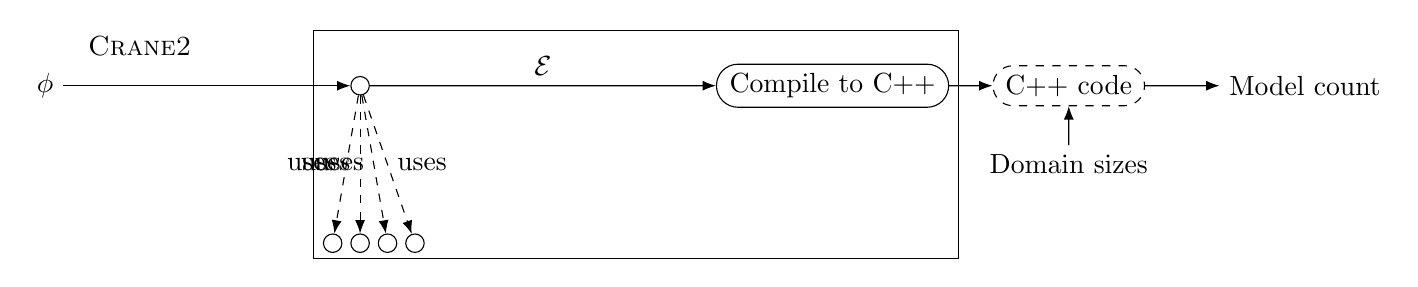
\begin{tikzpicture}
    \node at (-1, 0) (formula) {$\phi$};
    \node[draw,rounded rectangle] at (3, 0) (compilewithbasecases) {\CompileWithBaseCases};
    \node[draw,rounded rectangle] at (9, 0) (compilation) {Compile to C++};

    \node[draw,rounded rectangle,dashed] at (12, 0) (cpp) {C++ code};
    \node at (12, -1) (sizes) {Domain sizes};

    \node at (15, 0) (count) {Model count};

    \node[draw,rounded rectangle] at (3, -2) (findbasecases) {\FindBaseCases};
    \node[draw,rounded rectangle,left = 0.1cm of findbasecases] (crane) {\Compile};
    \node[draw,rounded rectangle,right = 0.1cm of findbasecases] (propagate) {\Propagate};
    \node[draw,rounded rectangle,right = 0.1cm of propagate] (simplify) {\Simplify};

    \node[draw,fit={(compilewithbasecases) (compilation) (crane) (findbasecases) (propagate)},inner ysep=7pt,yshift=5pt] {};
    \node at (0.2, 0.5) {\Cranetwo};

    \draw[-Latex] (formula) -- (compilewithbasecases);
    \draw[-Latex] (compilewithbasecases) -- node[above] {$\mathcal{E}$} (compilation);
    \draw[-Latex] (compilation) -- (cpp);
    \draw[-Latex] (sizes) -- (cpp);
    \draw[-Latex] (cpp) -- (count);

    \draw[-Latex,dashed] (compilewithbasecases) -- node[midway,left] {uses} (crane);
    \draw[-Latex,dashed] (compilewithbasecases) -- node[midway,left] {uses} (findbasecases);
    \draw[-Latex,dashed] (compilewithbasecases) -- node[midway,left] {uses} (propagate);
    \draw[-Latex,dashed] (compilewithbasecases) -- node[midway,right] {uses} (simplify);
  \end{tikzpicture}
  \caption[]{The outline of using \Cranetwo{} to compute the model count of a formula $\phi$. First, the formula is compiled into a set of equations, which are then used to create a C++ program. This program can be executed with different command line arguments to calculate the model count of $\phi$ for different domain sizes. To accomplish this, the \CompileWithBaseCases function employs several components:
    \begin{enumerate*}[label=(\roman*)]
      \item the knowledge compilation algorithm of \textsc{Crane}, referred to as \Compile,
      \item a procedure called \FindBaseCases, which identifies a sufficient set of base cases,
      \item a procedure called \Propagate, which constructs a formula corresponding to a given base case, and
      \item algebraic simplification techniques (denoted as \Simplify).
    \end{enumerate*}
  }\label{fig:overview}
\end{figure*}

\Cref{fig:overview} outlines the workflow of the new algorithm. In
\cref{sec:main}, we describe how \CompileWithBaseCases finds the base cases for
recursive functions by:
\begin{enumerate*}[label=(\roman*)]
  \item identifying a sufficient set of base cases for each function,
  \item constructing formulas corresponding to these base cases,
  and\label[step]{step2}
  \item recursing on these new formulas.
\end{enumerate*}
Then, \cref{sec:smoothing} explains post-processing techniques for FCGs and the
formulas from \cref{step2} above required to preserve the correct model count.
Next, \cref{sec:cpp} elucidates how function definitions encoding a solution to
a WFOMC problem are compiled into C++ programs.\footnote{The possibility of
  compiling WFOMC solutions to C++ programs has been previously
  considered~\cite{DBLP:conf/kr/KazemiP16}. However, the extent of formulas that
  could be handled was limited.} Finally, \cref{sec:experiments} presents two
experiments comparing \Cranetwo{} with other state-of-the-art WFOMC algorithms.

\section{Preliminaries}

In \cref{sec:logic}, we provide a summary of the basic principles of first-order
logic. Then, in \cref{sec:threelogics}, we formally define WFOMC and discuss the
distinctions between three variations of first-order logic that are utilised for
WFOMC.\@ Finally, in \cref{sec:algebra}, we introduce the terminology used to
describe the output of the original \textsc{Crane} algorithm, i.e., functions
and equations that define them.

We use $\mathbb{N}_{0}$ to represent the set of non-negative integers. In both
algebra and logic, we write $S\sigma$ to denote the application of a
\emph{substitution} $\sigma$ to an expression $S$, where
$\sigma = [x_{1} \mapsto y_{1}, x_{2} \mapsto y_{2}, \dots, x_{n} \mapsto y_{n}]$
signifies the replacement of all instances of $x_{i}$ with $y_{i}$ for all
$i = 1, \dots, n$.

\subsection{First-Order Logic}\label{sec:logic}

In this section, we will review the basic concepts of first-order logic as they
are used in first-order knowledge compilation algorithms. There are two key
differences between the logic used within such algorithms and the logic
supported as input. First, Skolemization~\cite{DBLP:conf/kr/BroeckMD14} is
employed to eliminate existential quantifiers by introducing additional
predicates. Second, the input formula is rewritten as a conjunction of clauses,
each of which is in \emph{prenex normal form}~\cite{hinman2018fundamentals}.

A \emph{formula} is a conjunction of clauses. A \emph{clause} is of the form
$\forall x_{1} \in \Delta_{1}\text{.}\forall x_{2} \in \Delta_{2}\dots\text{
}\forall x_{n} \in \Delta_{n}\text{.}\phi(x_{1}, x_{2}, \dots, x_{n})$, where
$\phi$ is a disjunction of literals that only contain variables
$x_{1}, \dots, x_{n}$ (and any constants). We say that a clause is a
\emph{(positive) unit clause} if
\begin{enumerate*}[label=(\roman*)]
  \item there is only one literal with a predicate, and
  \item it is a positive literal.
\end{enumerate*}
A \emph{literal} is either an atom (i.e., a \emph{positive} literal) or its
negation (i.e., a \emph{negative} literal). An \emph{atom} is either
\begin{enumerate*}[label=(\roman*)]
  \item $P(t_{1}, \dots, t_{m})$ for some predicate $P$ and terms
  $t_{1}, \dots, t_{m}$ (written as $P(\mathbf{t})$ for short) or
  \item $x=y$ for some terms $x$ and $y$.
\end{enumerate*}
An atom is \emph{ground} if it contains no variables, i.e., only constants. The
\emph{arity} of a predicate is the number of arguments it takes, i.e., $m$ in
the case of predicate $P$ mentioned above. When we want to denote a predicate
together with its arity, we write $P/m$. A \emph{term} is either a variable or a
constant. Throughout the paper, we will use set-theoretic notation, interpreting
a formula as a set of clauses and a clause as a set of literals. Moreover, for
readability, clauses written on separate lines are implicitly conjoined.

\subsection{WFOMC Algorithms and Their Logics}\label{sec:threelogics}

\begin{table*}[t]
  \centering
  \begin{tabular}{llclll}
    \toprule
    Logic & Sorts & Constants & Variables & Quantifiers & Additional atoms\\
    \midrule
    \FO & one or more & \cmark & unlimited & $\forall$, $\exists$ & $x = y$\\
    \Ctwo & one & \xmark & two & $\forall$, $\exists$, $\exists^{= k}$, $\exists^{\le k}$, $\exists^{\ge k}$ & ---\\
    \UFO & one & \xmark & two & $\forall$ & $|P| = m$\\
    \bottomrule
  \end{tabular}
  \caption[]{Comparison of three logics used in WFOMC based on the following aspects:
    \begin{enumerate*}[label=(\roman*)]
      \item number of sorts,
      \item support for constants,
      \item maximum number of variables,
      \item supported quantifiers, and
      \item supported atoms in addition to those of the form $P(\mathbf{t})$ for a predicate $P/n$ and $n$-tuple of terms $\mathbf{t}$.
    \end{enumerate*}
    Here:
    \begin{enumerate*}[label=(\roman*)]
      \item $k$ and $m$ are non-negative integers, with the latter depending on the domain size,
      \item $P$ represents a predicate, and
      \item $x$ and $y$ are terms.
    \end{enumerate*}
  }\label{tbl:logics}
\end{table*}

In \cref{tbl:logics}, we outline the differences among three first-order logics
commonly used in WFOMC:
\begin{enumerate*}[label=(\roman*)]
  \item \FO{} is the input format for
  \textsc{ForcLift}\footnote{\url{https://github.com/UCLA-StarAI/Forclift}} and
  its extensions
  \textsc{Crane}\footnote{\url{https://doi.org/10.5281/zenodo.8004077}} and
  \Cranetwo{};
  \item \Ctwo{} is often used in the literature on \textsc{FastWFOMC} and
  related
  methods~\cite{DBLP:journals/jair/Kuzelka21,DBLP:conf/aaai/MalhotraS22};
  \item \UFO{} is the input format supported by a private version of
  \textsc{FastWFOMC} obtained directly from the authors.
\end{enumerate*}
Note that the publicly available
version\footnote{\url{https://comp.nus.edu.sg/~tvanbr/software/fastwfomc.tar.gz}}
of \textsc{FastWFOMC} does not support any cardinality constraints. The notation
we use to refer to each logic is standard in the case of \Ctwo{}, new in the
case of \UFO{}, and redefined to be more specific in the case of \FO{}. All
three logics are function-free, and domains are always assumed to be finite.

In \FO{}, each term is assigned to a \emph{sort}, and each predicate $P/n$ is
assigned to a sequence of $n$ sorts. Each sort has its corresponding domain.
Most of these assignments to sorts are typically left implicit and can be
reconstructed from the quantifiers. For example, $\forall x,y \in \Delta\text{.
}P(x, y)$ implies that variables $x$ and $y$ have the same sort. On the other
hand, $\forall x \in \Delta\text{. }\forall y \in \Gamma\text{. } P(x, y)$
implies that $x$ and $y$ have different sorts, and it would be improper to
write, for example, $\forall x \in \Delta\text{. }\forall y \in \Gamma\text{.
} P(x, y) \lor x = y$. \FO{} is also the only logic to support constants,
formulas with more than two variables, and the equality predicate.

\begin{remark}
  In the case of \textsc{ForcLift} and its extensions, support for a formula as
  valid input does not imply that the algorithm can compile the formula into a
  circuit or graph suitable for lifted model counting. However, it is known that
  \textsc{ForcLift} compilation is guaranteed to succeed on any \FO{} formula
  without constants and with at most two
  variables~\cite{DBLP:conf/nips/Broeck11,DBLP:conf/kr/BroeckMD14}.
\end{remark}

\Ctwo{} and \UFO{} are single-sorted (i.e., all variables are quantified over
the same domain) and only include formulas with at most two variables and no
constants. Unlike \UFO{}, \Ctwo{} supports existential quantifiers, including
\emph{counting quantifiers}. For example, $\exists^{=1} x\text{. }\phi(x)$ means
that there exists \emph{exactly one} $x$ such that $\phi(x)$, and
$\exists^{\le 2} x\text{. }\phi(x)$ means that there exist \emph{at most two}
such $x$. The advantage \UFO{} brings over \Ctwo{} is the support for
\emph{(equality) cardinality constraints}. For example, $|P| = 3$ constrains all
models to have \emph{precisely three positive literals with the predicate $P$}.

\begin{definition}[Model]\label{def:model}
  Let $\phi$ be a formula in \FO{}. For each predicate $P/n$ in $\phi$, let
  ${(\Delta_{i}^{P})}_{i=1}^{n}$ be a list of the corresponding domains (which
  may not be distinct). Let $\sigma$ be a map from the domains of $\phi$ to
  their interpretations as sets, satisfying the following conditions:
  \begin{enumerate*}[label=(\roman*)]
    \item the sets are pairwise disjoint, and
    \item the constants in $\phi$ are included in the corresponding domains.
  \end{enumerate*}
  Then a \emph{structure} of $\phi$ (with respect to $\sigma$) is a set $M$ of
  ground literals defined by adding either $P(\mathbf{t})$ or
  $\neg P(\mathbf{t})$ for every predicate $P/n$ in $\phi$ and $n$-tuple
  $\mathbf{t} \in \prod_{i=1}^{n} \sigma(\Delta_{i}^{P})$. A structure is a
  \emph{model} if it satisfies $\phi$.
\end{definition}

\begin{definition}[WFOMC~\cite{DBLP:conf/ijcai/BroeckTMDR11}]
  Continuing from \cref{def:model}, for each predicate $P$ in $\phi$, let
  $w^{+}(P)$ and $w^{-}(P)$ be its \emph{weights} in $\mathbb{Q}$. Unless
  specified otherwise, we assume all weights are equal to one. The
  \emph{(symmetric) weighted first-order model count} (WFOMC) of $\phi$ (with
  respect to $\sigma$, $w^{+}$, and $w^{-}$) is:
  \[
    \sum_{M \models \phi} \prod_{P(\mathbf{t}) \in M} w^{+}(P) \prod_{\neg P(\mathbf{t}) \in M} w^{-}(P),
  \]
  where the sum is over all models of $\phi$.
\end{definition}

\begin{example}[Counting functions]\label{example:functions}
  To define predicate $P$ as an endofunction on $\Delta$, in \Ctwo{} one would
  write $\forall x \in \Delta\text{. }\exists^{=1} y \in \Delta\text{.
  }P(x, y)$. In \UFO{}, the same could be written as
  \begin{equation}\label[formula]{eq:functions1}
    \begin{gathered}
      \forall x, y \in \Delta\text{. }S(x) \lor \neg P(x, y)\\
      |P| = |\Delta|,
    \end{gathered}
  \end{equation}
  where $w^{-}(S) = -1$. Although \cref{eq:functions1} has more models compared
  to its counterpart in \Ctwo{}, the weight function makes the \emph{weighted}
  model count of \cref{eq:functions1} equal to the number of endofunctions on
  $\Delta$.

  Equivalently, in \FO{} we would write
  \begin{equation}\label[formula]{eq:fo}
    \begin{gathered}
      \forall x \in \Gamma\text{. }\exists y \in \Delta\text{. }P(x, y)\\
      \forall x \in \Gamma\text{. }\forall y, z \in \Delta\text{. }P(x, y) \land P(x, z) \Rightarrow y = z.
    \end{gathered}
  \end{equation}
  The first clause asserts that each $x$ must have at least one corresponding
  $y$, while the second statement adds the condition that if $x$ is mapped to
  both $y$ and $z$, then $y$ must equal $z$. It is important to note that
  \cref{eq:fo} is written with two domains instead of just one. However, we can
  still determine the number of endofunctions by assuming that the sizes of
  $\Gamma$ and $\Delta$ are equal. This formulation, as observed by Dilkas and
  Belle~\shortcite{DBLP:conf/kr/DilkasB23}, can prove beneficial in enabling
  first-order knowledge compilation algorithms to find efficient solutions.
\end{example}

\subsection{Algebra}\label{sec:algebra}

We write $\expr{}$ to represent an arbitrary algebraic expression. It is
important to note that some terms have different meanings in algebra compared to
logic. In algebra, a \emph{constant} refers to a non-negative integer. Likewise,
a \emph{variable} can either be a parameter of a function or a variable
introduced through summation, such as $i$ in the expression
$\sum_{i=1}^{n} \expr$. A (function) \emph{signature} is
$f(x_{1}, \dots, x_{n})$ (or $f(\mathbf{x})$ for short), where $f$ represents an
$n$-ary function, and each $x_{i}$ represents a variable. An \emph{equation} is
$f(\mathbf{x}) = \expr{}$, with $f(\mathbf{x})$ representing a signature.

\begin{definition}[Base case]\label{def:basecase}
  Let $f(\mathbf{x})$ be a function call where each $x_{i}$ is either a constant
  or a variable (note that signatures are included in this definition). Then
  function call $f(\mathbf{y})$ is considered a \emph{base case} of
  $f(\mathbf{x})$ if $f(\mathbf{y}) = f(\mathbf{x})\sigma$, where $\sigma$ is a
  substitution that replaces one or more $x_{i}$ with a constant.
\end{definition}

\section{Completing the Definitions of Recursive Functions}\label{sec:main}

\begin{algorithm}[t]
  \caption{\protect\CompileWithBaseCases{$\phi$}}\label{alg:compilewithbasecases}
  \KwIn{formula $\phi$}
  \KwOut{set $\mathcal{E}$ of equations}
  $(\mathcal{E}, \mathcal{F}, \mathcal{D}) \gets \Compile{$\phi$}$\;\label{line:first}
  $\mathcal{E} \gets \Simplify{$\mathcal{E}$}$\;\label{line:second}
  \ForEach{base case $f(\mathbf{x}) \in \FindBaseCases{$\mathcal{E}$}$}{
    $\psi \gets \mathcal{F}(f)$\;
    \ForEach{$i$ such that $x_{i} \in \mathbb{N}_{0}$}{
      $\psi \gets \Propagate{$\psi$, $\mathcal{D}(f, i)$, $x_i$}$\;
    }
    $\mathcal{E} \gets \mathcal{E} \cup \CompileWithBaseCases{$\psi$}$\;
  }
\end{algorithm}

\Cref{alg:compilewithbasecases} presents our overall approach for compiling a
formula into equations that include the necessary base cases. To begin, we
utilise the knowledge compilation algorithm from the original \textsc{Crane} to
compile the formula into three components:
\begin{enumerate*}[label=(\roman*)]
  \item set $\mathcal{E}$ of equations,
  \item map $\mathcal{F}$ from function names to formulas, and
  \item map $\mathcal{D}$ from function names and argument indices to domains.
\end{enumerate*}
After some algebraic simplification, $\mathcal{E}$ is then passed to the
\FindBaseCases procedure (explained in \cref{sec:identifying}), which identifies
the base cases that need to be defined. For each base case $f(\mathbf{x})$, we
determine the formula associated with the function name $f$ and simplify it
using the \Propagate procedure (explained in \cref{sec:simplifying}). The
algorithm then calls itself on these simplified formulas and adds the resulting
base case equations to $\mathcal{E}$. \Cref{example:overall} provides a more
detailed explanation of \cref{alg:compilewithbasecases}.

\begin{example}[Counting bijections]\label{example:overall}
  Consider the following formula (previously examined by Dilkas and
  Belle~\shortcite{DBLP:conf/kr/DilkasB23}) that defines predicate $P$ as a
  bijection between two sets $\Gamma$ and $\Delta$:
  \[
    \begin{gathered}
      \forall x \in \Gamma\text{. }\exists y \in \Delta\text{. }P(x, y)\\
      \forall y \in \Delta\text{. }\exists x \in \Gamma\text{. }P(x, y)\\
      \forall x \in \Gamma\text{. }\forall y, z \in \Delta\text{. }P(x, y) \land P(x, z) \Rightarrow y = z\\
      \forall x, z \in \Gamma\text{. }\forall y \in \Delta\text{. }P(x, y) \land P(z, y) \Rightarrow x = z.
    \end{gathered}
  \]
  We specifically examine the first solution returned by \Cranetwo{} for this
  formula.

  After \cref{line:first,line:second}, we have
  \begin{align*}
    \mathcal{E} &= \left\{\,\begin{aligned}f(m, n) &= \sum_{l=0}^{n} \binom{n}{l}{(-1)}^{n-l}g(l, m),\\ g(l, m) &= g(l-1, m) + mg(l-1, m-1)\end{aligned}\,\right\};\\
    \mathcal{D} &= \{\, (f, 1) \mapsto \Gamma, (f, 2) \mapsto \Delta, (g, 1) \mapsto \Delta^{\top}, (g, 2) \mapsto \Gamma \,\},
  \end{align*}
  where $\Delta^{\top}$ is a new domain introduced by \Compile. Then
  \FindBaseCases identifies two base cases: $g(0, m)$ and $g(l, 0)$. In both
  cases, \CompileWithBaseCases recurses on the formula $\mathcal{F}(g)$
  simplified by assuming that one of the domains is empty. In the first case, we
  recurse on the formula $\forall x \in \Gamma\text{. }S(x) \lor \neg S(x)$,
  where $S$ is a predicate introduced by Skolemization with weights
  $w^{+}(S) = 1$ and $w^{-}(S) = -1$. Hence, we obtain the base case
  $g(0, m) = 0^{m}$. In the case of $g(l, 0)$, \Propagate{$\psi$, $\Gamma$, $0$}
  returns an empty formula, resulting in $g(l, 0) = 1$.
\end{example}

It is worth noting that these base cases overlap when $l = m = 0$ but remain
consistent since $0^{0} = 1$. Generally, let $\phi$ be a formula with two
domains $\Gamma$ and $\Delta$, and let $n, m \in \mathbb{N}_{0}$. Then the WFOMC
of \Propagate{$\phi$, $\Delta$, $n$} assuming $|\Gamma| = m$ is the same as the
WFOMC of \Propagate{$\phi$, $\Gamma$, $m$} assuming $|\Delta| = n$.

Finally, we highlight the crucial role of the \Simplify procedure in simplifying
the algebraic pattern $\sum_{m=0}^{n}[a \le m \le b] f(m)$. Here:
\begin{enumerate*}[label=(\roman*)]
  \item $n$ is a variable,
  \item $a, b \in \mathbb{N}_{0}$ are constants,
  \item $f$ is an expression that may depend on $m$, and
  \item $[a \le m \le b] =
  \begin{cases}
    1 & \text{if $a \le m \le b$} \\
    0 & \text{otherwise}
  \end{cases}$ represents the Iverson bracket.
\end{enumerate*}
\Simplify transforms this pattern into
$f(a) + f(a+1) + \cdots + f(\min\{\, n, b \,\})$. For instance, in the case of
\cref{example:overall}, \Simplify transforms
$g(l, m) = \sum_{k=0}^{m}[0 \le k \le 1]\binom{m}{k}g(l-1, m-k)$ into the
simplified form mentioned above.

\subsection{Identifying a Sufficient Set of Base Cases}\label{sec:identifying}

\begin{algorithm}[t]
  \caption{\protect\FindBaseCases{$\mathcal{E}$}}\label{alg:findbasecases}
  \KwIn{set $\mathcal{E}$ of equations}
  \KwOut{set $\mathcal{B}$ of base cases}

  $\mathcal{B} \gets \emptyset$\;
  \ForEach{equation $(f(\mathbf{x}) = \expr{}) \in \mathcal{E}$}{
    \ForEach{function call $f(\mathbf{y}) \in \expr{}$}{\label{line:functioncall}
      \ForEach{$y_{i} \in \mathbf{y}$} {
        \uIf{$y_{i} \in \mathbb{N}_{0}$}{
          $\mathcal{B} \gets \mathcal{B} \cup \{\, f(\mathbf{x})[x_{i} \mapsto y_{i}] \,\}$\;
        }
        \ElseIf{$y_{i} = x_{i} - c_{i}$ for some $c_{i} \in \mathbb{N}_{0}$}{
          \For{$j \gets 0$ \KwTo $c_{i} - 1$}{\label{line:lim}
            $\mathcal{B} \gets \mathcal{B} \cup \{\, f(\mathbf{x})[x_{i} \mapsto j] \,\}$\;\label{line:insert}
          }
        }
      }
    }
  }
\end{algorithm}

\Cref{alg:findbasecases} summarises the implementation of the \FindBaseCases
function. When a function $f$ calls itself recursively, \FindBaseCases considers
two types of arguments:
\begin{enumerate*}[label=(\roman*)]
  \item constants and
  \item arguments of the form $x_{i} - c_{i}$, where $c_{i}$ is a constant and
  $x_{i}$ is the $i$-th argument of the signature of $f$.
\end{enumerate*}
If the argument is a constant $c_{i}$, a base case with $c_{i}$ is added. In the
second case, a base case is added for each constant from zero up to (but not
including) $c_{i}$. The following discussion explains the reasoning behind this
approach.

\begin{example}
  Let us consider the recursive function $g$ from \cref{example:overall}. In
  this case, \FindBaseCases iterates over two function calls: $g(l-1, m)$ and
  $g(l-1, m-1)$. The former produces the base case $g(0, m)$, while the latter
  produces both $g(0, m)$ and $g(l, 0)$.
\end{example}

For the rest of this section, let $\mathcal{E}$ represent the equations returned
by \CompileWithBaseCases. To demonstrate that the base cases identified by
\FindBaseCases are sufficient, we begin with a few observations that stem from
the details of previous
work~\cite{DBLP:conf/ijcai/BroeckTMDR11,DBLP:conf/kr/DilkasB23} and this work.

\begin{fact}\label{assumption1}
  For each function $f$, there is precisely one equation $e \in \mathcal{E}$
  with $f(\mathbf{x})$ on the left-hand side where all $x_{i}$'s are variables
  (i.e., $e$ is not a base case). We refer to $e$ as the \emph{definition} of
  $f$.
\end{fact}

\begin{fact}\label{assumption2}
  There is a \emph{topological ordering} of all functions ${(f_{i})}_{i}$ in
  $\mathcal{E}$ such that equations in $\mathcal{E}$ with $f_{i}$ on the
  left-hand side do not contain function calls to $f_{j}$ with $j > i$. This
  condition prevents mutual recursion and other cyclic scenarios.
\end{fact}

\begin{fact}\label{assumption3}
  For every equation $(f(\mathbf{x}) = \expr) \in \mathcal{E}$, the evaluation
  of $\expr$ terminates when provided with the values of all relevant function
  calls.
\end{fact}

\begin{corollary}\label{fact}
  If $f$ is a non-recursive function with no function calls on the right-hand
  side of its definition, then the evaluation of any function call
  $f(\mathbf{x})$ terminates.
\end{corollary}

\begin{fact}\label{fact2}
  For any equation $f(\mathbf{x}) = \expr{}$, if $\mathbf{x}$ contains only
  constants, then $\expr{}$ cannot include any function calls to $f$.
\end{fact}

Additionally, we introduce an assumption about the structure of recursion.

\begin{assumption}\label{assumption4}
  For every equation $(f(\mathbf{x}) = \expr) \in \mathcal{E}$, every recursive
  function call $f(\mathbf{y}) \in \expr$ satisfies the
  following:
  \begin{itemize}
    \item Each $y_{i}$ is either $x_{i} - c_{i}$ or $c_{i}$ for some constant
          $c_{i}$.
    \item There exists $i$ such that $y_{i} = x_{i} - c_{i}$ for some
          $c_{i} > 0$.
  \end{itemize}
\end{assumption}

Finally, we assume a particular order of evaluation for function calls using the
equations in $\mathcal{E}$. Specifically, we assume that base cases are
considered before the recursive definition. The exact order in which base cases
are considered is not relevant.

\begin{assumption}
  When multiple equations in $\mathcal{E}$ match a function call
  $f(\mathbf{x})$, preference is given to an equation with the most constants on
  its left-hand side.
\end{assumption}

With the facts and assumptions mentioned above, we prove the following theorem.

\begin{theorem}[Termination]\label{thm:halting}
  Let $f$ be an $n$-ary function in $\mathcal{E}$ and
  $\mathbf{x} \in \mathbf{N}_{0}^{n}$. Then the evaluation of $f(\mathbf{x})$
  terminates.
\end{theorem}

We prove \cref{thm:halting} using double induction. First, we apply induction on
the number of functions in $\mathcal{E}$. Then, we use induction on the arity of
the `last' function in $\mathcal{E}$ according to some topological ordering (as
defined in \cref{assumption2}). For readability, we divide the proof into
several lemmas of increasing generality.

\begin{lemma}\label{lemma:oneunary}
  Assume that $\mathcal{E}$ consists of just \emph{one unary} function $f$. Then
  the evaluation of a function call $f(x)$ terminates for any
  $x \in \mathbb{N}_{0}$.
\end{lemma}
\begin{proof}
  If $f(x)$ is captured by a base case, then its evaluation terminates by
  \cref{fact,fact2}. If $f$ is not recursive, the evaluation of
  $f(x)$ terminates by \cref{fact}.

  Otherwise, let $f(y)$ be an arbitrary function call on the right-hand side of
  the definition of $f(x)$. If $y$ is a constant, there is a base case for
  $f(y)$. Otherwise, let $y = x - c$ for some $c > 0$. Then there exists
  $k \in \mathbb{N}_{0}$ such that $0 \le x - kc \le c-1$. So, after $k$
  iterations, the sequence of function calls $f(x), f(x-c), f(x-2c),\dots$ will
  be captured by the base case $f(x \mod c)$.
\end{proof}

\begin{lemma}\label{lemma:onefunction}
  Generalising \cref{lemma:oneunary}, let $\mathcal{E}$ be a set of equations
  for \emph{one} $n$-ary function $f$ for some $n \ge 1$. Then the evaluation of
  $f(\mathbf{x})$ terminates for any $\mathbf{x} \in \mathbb{N}_{0}^{n}$.
\end{lemma}
\begin{proof}
  If $f$ is non-recursive, the evaluation of $f(\mathbf{x})$ terminates by
  previous arguments. We proceed by induction on $n$, with the base case of
  $n=1$ handled by \cref{lemma:oneunary}. Assume that $n > 1$. Any base case of
  $f$ can be seen as a function of arity $n-1$, since one of the parameters is
  fixed. Thus, the evaluation of any base case terminates by the inductive
  hypothesis. It remains to show that the evaluation of the recursive equation
  for $f$ terminates, but that follows from \cref{assumption3}.
\end{proof}

\begin{proof}[Proof of \cref{thm:halting}]
  We proceed by induction on the number of functions $n$. The base case of $n=1$
  is handled by \cref{lemma:onefunction}. Let ${(f_{i})}_{i=1}^{n}$ be some
  topological ordering of these $n > 1$ functions. If $f = f_{j}$ for $j < n$,
  then the evaluation of $f(\mathbf{x})$ terminates by the inductive hypothesis
  since $f_{j}$ cannot call $f_{n}$ by \cref{assumption2}. Using the inductive
  hypothesis that all function calls to $f_{j}$ (with $j < n$) terminate, the
  proof proceeds similarly to the Proof of \cref{lemma:onefunction}.
\end{proof}

\subsection{Propagating Domain Size Assumptions}\label{sec:simplifying}

\begin{algorithm}[t]
  \caption{\protect\Propagate{$\phi$, $\Delta$, $n$}}\label{alg:propagate}
  \KwIn{formula $\phi$, domain $\Delta$, $n \in \mathbb{N}_{0}$}
  \KwOut{formula $\phi'$}
  $\phi' \gets \emptyset$\;
  \uIf{$n = 0$}{
    \ForEach{clause $C \in \phi$}{
      \lIf{$\Delta \not\in \Doms(C)$}{$\phi' \gets \phi' \cup \{\, C \,\}$}
      \Else{
        $C' \gets \{\, l \in C \mid \Delta \not\in \Doms(l) \,\}$\;
        \If{$C' \ne \emptyset$}{
          $l \gets \text{an arbitrary literal in } C'$\;\label{line:smoothing1}
          $\phi' \gets \phi' \cup \{\, C' \cup \{\, \neg l \,\} \,\} $\;\label{line:smoothing2}
        }
      }
    }
  }
  \Else{
    $D \gets \text{a set of $n$ new constants in $\Delta$}$\;
    \ForEach{clause $C \in \phi$}{
      ${(x_{i})}_{i=1}^{m} \gets \text{the variables in $C$ with domain $\Delta$}$\;
      \lIf{$m = 0$}{$\phi' \gets \phi' \cup \{\, C \,\}$}
      \Else{
        $\phi' \gets \phi' \cup \{\, C[x_{1} \mapsto c_{1}, \dots, x_{m} \mapsto c_{m}] \mid {(c_{i})}_{i=1}^{m} \in D^{m} \,\}$\;
      }
    }
  }
\end{algorithm}

\Cref{alg:propagate}, called \Propagate, modifies the formula $\phi$ based on
the assumption that $|\Delta| = n$. When $n=0$, some clauses become vacuously
satisfied and can be removed. When $n > 0$\footnote{None of the formulas
  examined in this study had $n > 1$.}, partial grounding is performed by
replacing all variables quantified over $\Delta$ with constants.
\Cref{alg:propagate} handles these two cases separately. For a literal or a
clause $C$, the set of corresponding domains is denoted as $\Doms(C)$.

In the case of $n = 0$, there are three types of clauses to consider:
\begin{enumerate*}[label=(\roman*)]
  \item those that do not mention $\Delta$,\label[type]{type1}
  \item those in which every literal contains variables quantified over
  $\Delta$, and\label[type]{type2}
  \item those that have some literals with variables quantified over $\Delta$
  and some without.\label[type]{type3}
\end{enumerate*}
Clauses of \cref{type1} are transferred to the new formula $\phi'$ without any
changes. For clauses of \cref{type2}, $C'$ is empty, so these clauses are
filtered out. As for clauses of \cref{type3}, a new kind of smoothing is
performed, which will be explained in \cref{sec:smoothingbase}.

In the case of $n>0$, $n$ new constants are introduced. Let $C$ be an arbitrary
clause in $\phi$, and let $m \in \mathbb{N}_{0}$ be the number of variables in
$C$ quantified over $\Delta$. If $m=0$, $C$ is added directly to $\phi'$.
Otherwise, a clause is added to $\phi'$ for every possible combination of
replacing the $m$ variables in $C$ with the $n$ new constants.

\begin{example}
  Let $C \equiv \forall x \in \Gamma\text{. }\forall y, z \in \Delta\text{.
  } \neg P(x, y) \lor \neg P(x, z) \lor y=z$. Then
  $\Doms(C) = \Doms(\neg P(x, y)) = \Doms(\neg P(x, z)) = \{\, \Gamma, \Delta \,\}$,
  and $\Doms(y=z) = \{\, \Delta \,\}$. A call to \Propagate{$\{\, C \,\}$,
    $\Delta$, $3$} would result in the following formula with nine clauses:
  \begin{align*}
    \forall x \in \Gamma\text{. }\neg P(x, c_{1}) \lor& \neg P(x, c_{1}) \lor c_{1}=c_{1}\\
    \forall x \in \Gamma\text{. }\neg P(x, c_{1}) \lor& \neg P(x, c_{2}) \lor c_{1}=c_{2}\\
    \vdots&\\
    \forall x \in \Gamma\text{. }\neg P(x, c_{3}) \lor& \neg P(x, c_{3}) \lor c_{3}=c_{3}.\\
  \end{align*}
  Here, $c_{1}$, $c_{2}$, and $c_{3}$ are the new constants.
\end{example}

\section{Smoothing}\label{sec:smoothing}

\emph{Smoothness} is a property originating in propositional knowledge
compilation, where it refers to the situation where all disjuncts in a
disjunction node contain the same atoms~\cite{darwiche2001tractable}. Van den
Broeck et al.~\shortcite{DBLP:conf/ijcai/BroeckTMDR11} extend this concept to
first-order logic, introducing set-disjunction and inclusion-exclusion nodes in
addition to disjunction.

The purpose of smoothing is as follows. When compilation rules such as unit
propagation and inclusion-exclusion simplify a formula, certain ground atoms may
be eliminated (see \cref{example:basecasesmoothing} below). To properly account
for these atoms during counting, smoothing nodes (i.e., tautological clauses
such as $P(c) \lor \neg P(c)$) are added to the FCG in the appropriate location.

The remainder of this section presents an extension to the smoothing algorithm
of Van den Broeck et al.~\shortcite{DBLP:conf/ijcai/BroeckTMDR11}.
\Cref{sec:smoothingbase} explains the role of smoothing in the base-case-finding
algorithm described in \cref{sec:main}. \Cref{sec:smoothingfcg1} demonstrates
how to adapt smoothing to the compilation rules introduced by Dilkas and
Belle~\shortcite{DBLP:conf/kr/DilkasB23}.

\subsection{Smoothing for Base Cases}\label{sec:smoothingbase}

In this section, we motivate and describe \cref{line:smoothing1,line:smoothing2}
of \cref{alg:propagate}. Suppose that \Propagate is called with arguments
$(\phi, \Delta, 0)$, which means we are simplifying the formula $\phi$ by
assuming that the domain $\Delta$ is empty. Informally, if there is a predicate
$P$ in $\phi$ that has nothing to do with the domain $\Delta$, smoothing
preserves all occurrences of $P$ even if all clauses with $P$ become vacuously
satisfied. It is important to note that the approach presented in this section
is not unique. We explain it via the example below.

\begin{example}\label{example:basecasesmoothing}
  Let $\phi$ be:
  \begin{align}
    \forall x \in \Delta\text{. }\forall y, z \in \Gamma&\text{. }Q(x) \lor P(y, z)\label[clause]{eq:example1}\\
    \forall y, z \in \Gamma'&\text{. }P(y, z)\label[clause]{eq:example2},
  \end{align}
  where $\Gamma' \subseteq \Gamma$ is a domain introduced by a compilation rule.
  It should be noted that $P$, as a relation, is a subset of
  $\Gamma \times \Gamma$.

  Now, let us reason manually about the model count of $\phi$ when
  $\Delta = \emptyset$. Predicate $Q$ can only take one value, $Q = \emptyset$.
  The value of $P$ is fixed over $\Gamma' \times \Gamma'$ by \cref{eq:example2},
  but it is allowed to vary freely over
  $(\Gamma \times \Gamma) \setminus (\Gamma' \times \Gamma')$ since
  \cref{eq:example1} is vacuously satisfied by all structures. Therefore, the
  correct WFOMC should be $2^{|\Gamma|^2 - |\Gamma'|^2}$.

  However, without \cref{line:smoothing2}, \Propagate would simplify $\phi$ to
  $\forall y, z \in \Gamma'\text{. }P(y, z)$. In this case, $P$ is a subset of
  $\Gamma' \times \Gamma'$. This simplified formula has only one model:
  $\{\, P(y, z) \mid y, z \in \Gamma' \,\}$.

  By including \cref{line:smoothing2}, \Propagate transforms $\phi$ to:
  \begin{gather*}
    \forall y, z \in \Gamma\text{. }P(y, z) \lor \neg P(y, z)\\
    \forall y, z \in \Gamma'\text{. }P(y, z),
  \end{gather*}
  which retains the correct model count.
\end{example}

It is worth mentioning that the choice of $l$ on \cref{line:smoothing1} of
\cref{alg:propagate} is inconsequential because any choice achieves the same
goal: constructing a tautological clause that retains the literals in $C'$.

\subsection{Smoothing the FCG}\label{sec:smoothingfcg1}

Smoothing is a two-step process that involves propagating unit clauses upwards
(i.e., in the opposite direction of FCG arcs) and adding smoothing nodes to
account for missing atoms. In this section, we will
\begin{enumerate*}[label=(\roman*)]
  \item describe the relevant node types from previous work,
  \item explain how smoothing should work for these node types, and
  \item demonstrate the new smoothing techniques using two example FCGs.
\end{enumerate*}

Before discussing the proposed changes to smoothing, let us briefly review the
compilation rules and their corresponding node types introduced by Dilkas and
Belle~\shortcite{DBLP:conf/kr/DilkasB23}. \emph{Domain recursion} involves
selecting a domain $\Delta$, introducing a new constant $c \in \Delta$, and
modifying the formula based on two possibilities for each variable $x$
quantified over $\Delta$: $x = c$ or $x \ne c$. The resulting node is denoted as
$\DR(c \in \Delta)$. \emph{Constraint removal} applies to formulas where each
variable $x$ quantified over a domain $\Delta$ is followed by the inequality
constraint $x \ne c$. These formulas can be rewritten so that each clause begins
with $\forall x \in \Delta\text{. }x \ne c \Rightarrow \ldots$ Constraint
removal replaces $\Delta$ with a new domain $\Delta'$ and removes the $x \ne c$
constraints. The resulting node is denoted as
$\CR(\Delta' \gets \Delta \setminus \{\,c\,\})$. Finally, \emph{caching} detects
when the input formula $\phi$ is equal to a previously encountered formula
$\psi$ except for having different domains. The resulting node is denoted as
$\Reff(\sigma)$, with $\sigma$ representing the substitution mapping the domains
of $\psi$ to their corresponding domains in $\phi$.

\paragraph{Stage~1 for Domain Recursion}
When visiting a $\DR(c \in \Delta)$ node, we replace each occurrence of
$\phi(c)$ or $\forall x \in \Delta\text{. } x \ne c \Rightarrow \phi(x)$ with
$\forall x \in \Delta\text{. }\phi(x)$ for each unit clause received from the
child node. This way, we ensure that if the subgraph below the domain recursion
node covers some of the ground atoms affected by domain recursion, it covers all
of them. If the relevant subgraph already covers those ground atoms, Stage~2
will not make any changes. Otherwise, smoothing nodes will be added below the
domain recursion node to account for the difference in the sets of ground atoms
assigned to the domain recursion node and its child node.

\paragraph{Stage~1 for Constraint Removal and Caching}
When visiting a $\CR(\Delta' \gets \Delta \setminus \{\,c\,\})$ node, we reverse
constraint removal by replacing each $\forall x \in \Delta'\text{. }\phi(x)$
with $\forall x \in \Delta\text{. }x \ne c \Rightarrow \phi(x)$. When visiting a
$\Reff(\sigma)$ node, we apply the substitution $\sigma$ to the unit clauses
from the child node.

\paragraph{Stage~2 for Domain Recursion}
We do not need to add smoothing nodes immediately below constraint removal or
caching nodes. However, for domain recursion, we follow a specific process.
\begin{enumerate}
  \item If the set of unit clauses assigned to the child node during Stage~1
        contains both $\phi(c)$ and $\forall x \in \Delta\text{.
        } x \ne c \Rightarrow \phi(x)$, we merge the two clauses into
        $\forall x \in \Delta\text{. }\phi(x)$. The only difference between
        these two clauses is that one has the constant $c$ while the other has a
        variable $x \ne c$.
  \item If necessary, we add smoothing nodes below the domain recursion node to
        account for the difference between the unit clauses assigned to the
        domain recursion node during Stage~1 and the unit clauses of the child
        node post-processed by the step above.
\end{enumerate}

\begin{figure}[t]
  \centering
  \begin{forest}
    for tree={sn edges}
    [$\DR(c \in \Delta)$,name=dr,ellipse,draw
    [$\land$,ellipse,draw,dashed,edge=dashed
    [$P(c)$,rectangle,draw,fill=green!20]
    [$\forall x \in \Delta\text{. }x \ne c \Rightarrow P(x) \lor \neg P(x)$,rectangle,dashed,edge=dashed,draw,fill=blue!20]
    ]
    ]
  \end{forest}
  \caption{An artificial example of an FCG where a smoothing node needs to be
    added below a domain recursion node. The dashed nodes and arcs are added
    during Stage~2 of smoothing.}\label{fig:smoothing2}
\end{figure}

\begin{example}[An FCG that requires smoothing]
  \Cref{fig:smoothing2} depicts an FCG with a domain recursion node
  $\DR(c \in \Delta)$ followed directly by a single $P(c)$ node. In this
  scenario, Stage~1 assigns $\{\, \forall x \in \Delta\text{. }P(x) \,\}$ to the
  former node and $\{\, P(c) \,\}$ to the latter. As these two sets of unit
  clauses cover different ground atoms, Stage~2 adds a smoothing node to address
  $P(x)$ for all $x \in \Delta \setminus \{\, c \,\}$.
\end{example}

\begin{figure}[t]
  \centering
  \begin{forest}
    for tree={sn edges}
    [$\DR(c \in \Delta)$,name=dr,ellipse,draw,label={right:\textcolor{blue}{3. $\{\, \forall x \in \Delta\text{. }P(x) \,\}$}}
    [$\land$,ellipse,draw,label={left:\textcolor{blue}{2. $\{\, P(c) \,\}$}},label={right:\textcolor{blue}{6. $\{\, P(c), \forall x \in \Delta\text{. }x \ne c \Rightarrow P(x) \,\}$}}
    [$P(c)$,rectangle,draw,fill=green!20,label={272:\textcolor{blue}{1. $\{\, P(c) \,\}$}}]
    [$\CR(\Delta' \gets \Delta \setminus \{\, c \,\})$,ellipse,draw,label={87:\textcolor{blue}{5. $\{\, \forall x \in \Delta\text{. }x \ne c \Rightarrow P(x) \,\}$}}
    [$\Reff(\Delta \mapsto \Delta')$,name=ref,ellipse,draw,label={below:\textcolor{blue}{4. $\{\, \forall x \in \Delta'\text{. }P(x) \,\}$}}]
    ]
    ]
    ]
  \end{forest}
  \caption{A smooth FCG based on \cref{example:overall}. For compactness, the
    arc between the caching node and the domain recursion node is not shown. The
    labels next to the nodes indicate the sets of unit clauses assigned to each
    node during Stage~1 and the order in which these assignments were made.
    Empty assignments that replace a set $S$ with $S$ itself are not
    included.}\label{fig:smoothing1}
\end{figure}

\begin{example}[A smooth FCG]\label{example:smooth}
  Stage~1 of the smoothing process is more complex in the case of the FCG shown
  in \cref{fig:smoothing1}. The unit clause $P(c)$ propagates to the conjunction
  node and is then generalised to $\forall x \in \Delta\text{. }P(x)$ by the
  domain recursion node. It continues to propagate to the caching node, changing
  its form to $(\forall x \in \Delta\text{.
  }P(x))[\Delta \mapsto \Delta'] \equiv \forall x \in \Delta'\text{. }P(x)$. The
  constraint removal node re-introduces the constraints, transforming the clause
  to $\forall x \in \Delta\text{. }x \ne c \Rightarrow P(x)$, which then
  propagates to the conjunction node, joining $P(c)$.

  During Stage~2, $P(c)$ and $\forall x \in \Delta\text{.
  }x \ne c \Rightarrow P(x)$ are combined into $\forall x \in \Delta\text{.
  }P(x)$. Since the resulting clause matches the clause assigned to the domain
  recursion node, the FCG is already smooth.
\end{example}

The algebraic interpretation of \cref{fig:smoothing1} is an equation $e$ that
defines a recursive function. The right-hand side of $e$ already encompasses
$P(c)$, and the smoothing algorithm correctly recognises that the recursive call
also encompasses $P(x)$ for all $x \in \Delta \setminus \{\, c \,\}$.

\section{Generating C++ Code}\label{sec:cpp}

In this section, we will describe the final step of \Cranetwo{} as outlined in
\cref{fig:overview}. This step involves translating the set of equations
$\mathcal{E}$ into C++ code. The resulting C++ program can then be compiled and
executed with different command-line arguments to compute the model count of the
formula for various domain sizes.

Each equation in $\mathcal{E}$ is compiled into a C++ function, along with a
separate cache for memoisation. Let us consider an arbitrary equation
$e = (f(\mathbf{x}) = \expr{}) \in \mathcal{E}$, and let
$\mathbf{c} \in \mathbb{N}_{0}^{n}$ represent the arguments of the corresponding
C++ function. The implementation of $e$ consists of three parts. First, we check
if $\mathbf{c}$ is already present in the cache of $e$. If it is, we simply
return the cached value. Second, for each base case $f(\mathbf{y})$ of
$f(\mathbf{x})$ (as defined in \cref{def:basecase}), we check if $\mathbf{c}$
\emph{matches} $\mathbf{y}$, i.e., $c_{i} = y_{i}$ whenever
$y_{i} \in \mathbb{N}_{0}$. If this condition is satisfied, $\mathbf{c}$ is
redirected to the C++ function that corresponds to the definition of the base
case $f(\mathbf{y})$. Finally, if none of the above cases apply, we evaluate
$\mathbf{c}$ based on the expression $\expr{}$, store the result in the cache,
and return it.

\section{Experimental Evaluation}\label{sec:experiments}

We compared \Cranetwo{}\footnote{\textsc{Crane} has two modes that decide how
  compilation rules are applied to formulas: one that uses greedy search and
  another that combines greedy and breadth-first search. In our experiments, we
  refer to these modes as \Cranegreedy{} and \Cranebfs{}, respectively.} with
\textsc{FastWFOMC} and \textsc{ForcLift} on two problems previously considered
by Dilkas and Belle~\shortcite{DBLP:conf/kr/DilkasB23}. The first problem is the
function-counting problem from \cref{example:functions}, and the second problem
is the bijection-counting problem described below. It is important to note that
comparing \Cranetwo{} and \textsc{FastWFOMC} on a more substantial set of
benchmarks is challenging because there is no automated way to translate a
formula in \FO{} or \Ctwo{} into \UFO{}, or even check if such an encoding is
possible. We ran the experiments on an AMD~Ryzen~7~5800H processor with
\SI{16}{\gibi\byte} of memory and Arch Linux~6.8.2-arch2-1 operating system.
\textsc{FastWFOMC} was executed using Python~3.8.19 with Python-FLINT~0.5.0.

The \FO{} formula for bijections is described in \cref{example:overall}. The
equivalent formula in \Ctwo{} is
\begin{gather*}
  \forall x \in \Delta\text{. }\exists^{=1} y \in \Delta\text{. }P(x, y)\\
  \forall y \in \Delta\text{. }\exists^{=1} x \in \Delta\text{. }P(x, y).
\end{gather*}
Similarly, in \UFO{} the same formula can be written as
\begin{gather*}
  \forall x, y \in \Delta\text{. }R(x) \lor \neg P(x, y)\\
  \forall x, y \in \Delta\text{. }S(x) \lor \neg P(y, x)\\
  |P| = |\Delta|,
\end{gather*}
where $w^{-}(R) = w^{-}(S) = -1$.

\begin{figure}[t]
  \centering
  % Created by tikzDevice version 0.12.6 on 2024-08-15 12:12:55
% !TEX encoding = UTF-8 Unicode
\documentclass[10pt]{article}
\usepackage{tikz}

\usepackage[active,tightpage,psfixbb]{preview}

\PreviewEnvironment{pgfpicture}

\setlength\PreviewBorder{0pt}
\begin{document}

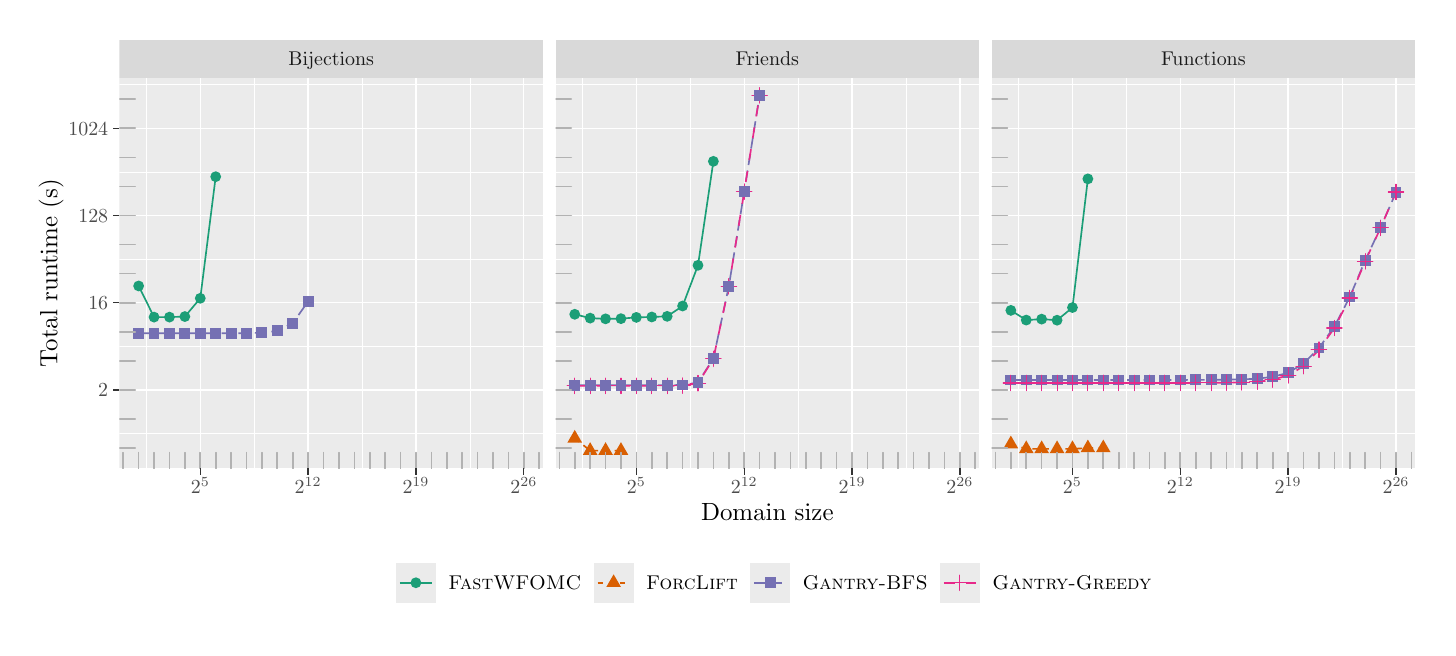
\begin{tikzpicture}[x=1pt,y=1pt]
\definecolor{fillColor}{RGB}{255,255,255}
\path[use as bounding box,fill=fillColor,fill opacity=0.00] (0,0) rectangle (505.89,216.81);
\begin{scope}
\path[clip] (  0.00,  0.00) rectangle (505.89,216.81);
\definecolor{drawColor}{RGB}{255,255,255}
\definecolor{fillColor}{RGB}{255,255,255}

\path[draw=drawColor,line width= 0.5pt,line join=round,line cap=round,fill=fillColor] ( -0.00,  0.00) rectangle (505.89,216.81);
\end{scope}
\begin{scope}
\path[clip] ( 33.14, 57.56) rectangle (186.23,198.75);
\definecolor{fillColor}{gray}{0.92}

\path[fill=fillColor] ( 33.14, 57.56) rectangle (186.23,198.75);
\definecolor{drawColor}{RGB}{255,255,255}

\path[draw=drawColor,line width= 0.2pt,line join=round] ( 33.14, 70.17) --
	(186.23, 70.17);

\path[draw=drawColor,line width= 0.2pt,line join=round] ( 33.14,101.68) --
	(186.23,101.68);

\path[draw=drawColor,line width= 0.2pt,line join=round] ( 33.14,133.19) --
	(186.23,133.19);

\path[draw=drawColor,line width= 0.2pt,line join=round] ( 33.14,164.70) --
	(186.23,164.70);

\path[draw=drawColor,line width= 0.2pt,line join=round] ( 33.14,196.21) --
	(186.23,196.21);

\path[draw=drawColor,line width= 0.2pt,line join=round] ( 42.89, 57.56) --
	( 42.89,198.75);

\path[draw=drawColor,line width= 0.2pt,line join=round] ( 81.85, 57.56) --
	( 81.85,198.75);

\path[draw=drawColor,line width= 0.2pt,line join=round] (120.82, 57.56) --
	(120.82,198.75);

\path[draw=drawColor,line width= 0.2pt,line join=round] (159.78, 57.56) --
	(159.78,198.75);

\path[draw=drawColor,line width= 0.5pt,line join=round] ( 33.14, 85.92) --
	(186.23, 85.92);

\path[draw=drawColor,line width= 0.5pt,line join=round] ( 33.14,117.43) --
	(186.23,117.43);

\path[draw=drawColor,line width= 0.5pt,line join=round] ( 33.14,148.95) --
	(186.23,148.95);

\path[draw=drawColor,line width= 0.5pt,line join=round] ( 33.14,180.46) --
	(186.23,180.46);

\path[draw=drawColor,line width= 0.5pt,line join=round] ( 62.37, 57.56) --
	( 62.37,198.75);

\path[draw=drawColor,line width= 0.5pt,line join=round] (101.34, 57.56) --
	(101.34,198.75);

\path[draw=drawColor,line width= 0.5pt,line join=round] (140.30, 57.56) --
	(140.30,198.75);

\path[draw=drawColor,line width= 0.5pt,line join=round] (179.27, 57.56) --
	(179.27,198.75);
\definecolor{drawColor}{RGB}{27,158,119}

\path[draw=drawColor,line width= 0.6pt,line join=round] ( 40.10,123.48) --
	( 45.67,112.22) --
	( 51.24,112.22) --
	( 56.80,112.42) --
	( 62.37,119.02) --
	( 67.94,162.96);
\definecolor{drawColor}{RGB}{117,112,179}

\path[draw=drawColor,line width= 0.6pt,dash pattern=on 4pt off 2pt ,line join=round] ( 40.10,106.36) --
	( 45.67,106.36) --
	( 51.24,106.36) --
	( 56.80,106.36) --
	( 62.37,106.36) --
	( 67.94,106.37) --
	( 73.50,106.38) --
	( 79.07,106.42) --
	( 84.64,106.58) --
	( 90.20,107.23) --
	( 95.77,109.99) --
	(101.34,117.90);
\definecolor{fillColor}{RGB}{117,112,179}

\path[fill=fillColor] ( 38.14,104.40) --
	( 42.06,104.40) --
	( 42.06,108.33) --
	( 38.14,108.33) --
	cycle;

\path[fill=fillColor] ( 43.71,104.40) --
	( 47.63,104.40) --
	( 47.63,108.33) --
	( 43.71,108.33) --
	cycle;

\path[fill=fillColor] ( 49.27,104.40) --
	( 53.20,104.40) --
	( 53.20,108.33) --
	( 49.27,108.33) --
	cycle;

\path[fill=fillColor] ( 54.84,104.40) --
	( 58.76,104.40) --
	( 58.76,108.33) --
	( 54.84,108.33) --
	cycle;

\path[fill=fillColor] ( 60.41,104.40) --
	( 64.33,104.40) --
	( 64.33,108.33) --
	( 60.41,108.33) --
	cycle;

\path[fill=fillColor] ( 65.97,104.40) --
	( 69.90,104.40) --
	( 69.90,108.33) --
	( 65.97,108.33) --
	cycle;

\path[fill=fillColor] ( 71.54,104.41) --
	( 75.46,104.41) --
	( 75.46,108.34) --
	( 71.54,108.34) --
	cycle;

\path[fill=fillColor] ( 77.11,104.45) --
	( 81.03,104.45) --
	( 81.03,108.38) --
	( 77.11,108.38) --
	cycle;

\path[fill=fillColor] ( 82.67,104.62) --
	( 86.60,104.62) --
	( 86.60,108.54) --
	( 82.67,108.54) --
	cycle;

\path[fill=fillColor] ( 88.24,105.27) --
	( 92.16,105.27) --
	( 92.16,109.19) --
	( 88.24,109.19) --
	cycle;

\path[fill=fillColor] ( 93.81,108.02) --
	( 97.73,108.02) --
	( 97.73,111.95) --
	( 93.81,111.95) --
	cycle;

\path[fill=fillColor] ( 99.37,115.94) --
	(103.30,115.94) --
	(103.30,119.87) --
	( 99.37,119.87) --
	cycle;
\definecolor{fillColor}{RGB}{27,158,119}

\path[fill=fillColor] ( 40.10,123.48) circle (  1.96);

\path[fill=fillColor] ( 45.67,112.22) circle (  1.96);

\path[fill=fillColor] ( 51.24,112.22) circle (  1.96);

\path[fill=fillColor] ( 56.80,112.42) circle (  1.96);

\path[fill=fillColor] ( 62.37,119.02) circle (  1.96);

\path[fill=fillColor] ( 67.94,162.96) circle (  1.96);
\definecolor{drawColor}{gray}{0.70}

\path[draw=drawColor,line width= 0.6pt,line join=round,line cap=round] ( 34.54, 57.56) -- ( 34.54, 63.25);

\path[draw=drawColor,line width= 0.6pt,line join=round,line cap=round] ( 40.10, 57.56) -- ( 40.10, 63.25);

\path[draw=drawColor,line width= 0.6pt,line join=round,line cap=round] ( 45.67, 57.56) -- ( 45.67, 63.25);

\path[draw=drawColor,line width= 0.6pt,line join=round,line cap=round] ( 51.24, 57.56) -- ( 51.24, 63.25);

\path[draw=drawColor,line width= 0.6pt,line join=round,line cap=round] ( 56.80, 57.56) -- ( 56.80, 63.25);

\path[draw=drawColor,line width= 0.6pt,line join=round,line cap=round] ( 62.37, 57.56) -- ( 62.37, 63.25);

\path[draw=drawColor,line width= 0.6pt,line join=round,line cap=round] ( 67.94, 57.56) -- ( 67.94, 63.25);

\path[draw=drawColor,line width= 0.6pt,line join=round,line cap=round] ( 73.50, 57.56) -- ( 73.50, 63.25);

\path[draw=drawColor,line width= 0.6pt,line join=round,line cap=round] ( 79.07, 57.56) -- ( 79.07, 63.25);

\path[draw=drawColor,line width= 0.6pt,line join=round,line cap=round] ( 84.64, 57.56) -- ( 84.64, 63.25);

\path[draw=drawColor,line width= 0.6pt,line join=round,line cap=round] ( 90.20, 57.56) -- ( 90.20, 63.25);

\path[draw=drawColor,line width= 0.6pt,line join=round,line cap=round] ( 95.77, 57.56) -- ( 95.77, 63.25);

\path[draw=drawColor,line width= 0.6pt,line join=round,line cap=round] (101.34, 57.56) -- (101.34, 63.25);

\path[draw=drawColor,line width= 0.6pt,line join=round,line cap=round] (106.90, 57.56) -- (106.90, 63.25);

\path[draw=drawColor,line width= 0.6pt,line join=round,line cap=round] (112.47, 57.56) -- (112.47, 63.25);

\path[draw=drawColor,line width= 0.6pt,line join=round,line cap=round] (118.04, 57.56) -- (118.04, 63.25);

\path[draw=drawColor,line width= 0.6pt,line join=round,line cap=round] (123.60, 57.56) -- (123.60, 63.25);

\path[draw=drawColor,line width= 0.6pt,line join=round,line cap=round] (129.17, 57.56) -- (129.17, 63.25);

\path[draw=drawColor,line width= 0.6pt,line join=round,line cap=round] (134.74, 57.56) -- (134.74, 63.25);

\path[draw=drawColor,line width= 0.6pt,line join=round,line cap=round] (140.30, 57.56) -- (140.30, 63.25);

\path[draw=drawColor,line width= 0.6pt,line join=round,line cap=round] (145.87, 57.56) -- (145.87, 63.25);

\path[draw=drawColor,line width= 0.6pt,line join=round,line cap=round] (151.44, 57.56) -- (151.44, 63.25);

\path[draw=drawColor,line width= 0.6pt,line join=round,line cap=round] (157.00, 57.56) -- (157.00, 63.25);

\path[draw=drawColor,line width= 0.6pt,line join=round,line cap=round] (162.57, 57.56) -- (162.57, 63.25);

\path[draw=drawColor,line width= 0.6pt,line join=round,line cap=round] (168.13, 57.56) -- (168.13, 63.25);

\path[draw=drawColor,line width= 0.6pt,line join=round,line cap=round] (173.70, 57.56) -- (173.70, 63.25);

\path[draw=drawColor,line width= 0.6pt,line join=round,line cap=round] (179.27, 57.56) -- (179.27, 63.25);

\path[draw=drawColor,line width= 0.6pt,line join=round,line cap=round] (184.83, 57.56) -- (184.83, 63.25);

\path[draw=drawColor,line width= 0.6pt,line join=round,line cap=round] ( 33.14, 64.92) -- ( 38.84, 64.92);

\path[draw=drawColor,line width= 0.6pt,line join=round,line cap=round] ( 33.14, 75.42) -- ( 38.84, 75.42);

\path[draw=drawColor,line width= 0.6pt,line join=round,line cap=round] ( 33.14, 85.92) -- ( 38.84, 85.92);

\path[draw=drawColor,line width= 0.6pt,line join=round,line cap=round] ( 33.14, 96.43) -- ( 38.84, 96.43);

\path[draw=drawColor,line width= 0.6pt,line join=round,line cap=round] ( 33.14,106.93) -- ( 38.84,106.93);

\path[draw=drawColor,line width= 0.6pt,line join=round,line cap=round] ( 33.14,117.43) -- ( 38.84,117.43);

\path[draw=drawColor,line width= 0.6pt,line join=round,line cap=round] ( 33.14,127.94) -- ( 38.84,127.94);

\path[draw=drawColor,line width= 0.6pt,line join=round,line cap=round] ( 33.14,138.44) -- ( 38.84,138.44);

\path[draw=drawColor,line width= 0.6pt,line join=round,line cap=round] ( 33.14,148.95) -- ( 38.84,148.95);

\path[draw=drawColor,line width= 0.6pt,line join=round,line cap=round] ( 33.14,159.45) -- ( 38.84,159.45);

\path[draw=drawColor,line width= 0.6pt,line join=round,line cap=round] ( 33.14,169.95) -- ( 38.84,169.95);

\path[draw=drawColor,line width= 0.6pt,line join=round,line cap=round] ( 33.14,180.46) -- ( 38.84,180.46);

\path[draw=drawColor,line width= 0.6pt,line join=round,line cap=round] ( 33.14,190.96) -- ( 38.84,190.96);
\end{scope}
\begin{scope}
\path[clip] (190.73, 57.56) rectangle (343.81,198.75);
\definecolor{fillColor}{gray}{0.92}

\path[fill=fillColor] (190.73, 57.56) rectangle (343.81,198.75);
\definecolor{drawColor}{RGB}{255,255,255}

\path[draw=drawColor,line width= 0.2pt,line join=round] (190.73, 70.17) --
	(343.81, 70.17);

\path[draw=drawColor,line width= 0.2pt,line join=round] (190.73,101.68) --
	(343.81,101.68);

\path[draw=drawColor,line width= 0.2pt,line join=round] (190.73,133.19) --
	(343.81,133.19);

\path[draw=drawColor,line width= 0.2pt,line join=round] (190.73,164.70) --
	(343.81,164.70);

\path[draw=drawColor,line width= 0.2pt,line join=round] (190.73,196.21) --
	(343.81,196.21);

\path[draw=drawColor,line width= 0.2pt,line join=round] (200.47, 57.56) --
	(200.47,198.75);

\path[draw=drawColor,line width= 0.2pt,line join=round] (239.43, 57.56) --
	(239.43,198.75);

\path[draw=drawColor,line width= 0.2pt,line join=round] (278.40, 57.56) --
	(278.40,198.75);

\path[draw=drawColor,line width= 0.2pt,line join=round] (317.37, 57.56) --
	(317.37,198.75);

\path[draw=drawColor,line width= 0.5pt,line join=round] (190.73, 85.92) --
	(343.81, 85.92);

\path[draw=drawColor,line width= 0.5pt,line join=round] (190.73,117.43) --
	(343.81,117.43);

\path[draw=drawColor,line width= 0.5pt,line join=round] (190.73,148.95) --
	(343.81,148.95);

\path[draw=drawColor,line width= 0.5pt,line join=round] (190.73,180.46) --
	(343.81,180.46);

\path[draw=drawColor,line width= 0.5pt,line join=round] (219.95, 57.56) --
	(219.95,198.75);

\path[draw=drawColor,line width= 0.5pt,line join=round] (258.92, 57.56) --
	(258.92,198.75);

\path[draw=drawColor,line width= 0.5pt,line join=round] (297.88, 57.56) --
	(297.88,198.75);

\path[draw=drawColor,line width= 0.5pt,line join=round] (336.85, 57.56) --
	(336.85,198.75);
\definecolor{drawColor}{RGB}{27,158,119}

\path[draw=drawColor,line width= 0.6pt,line join=round] (197.68,113.24) --
	(203.25,111.85) --
	(208.82,111.59) --
	(214.38,111.66) --
	(219.95,112.12) --
	(225.52,112.27) --
	(231.08,112.50) --
	(236.65,116.23) --
	(242.22,130.94) --
	(247.78,168.51);
\definecolor{drawColor}{RGB}{217,95,2}

\path[draw=drawColor,line width= 0.6pt,dash pattern=on 2pt off 2pt ,line join=round] (197.68, 68.42) --
	(203.25, 63.98) --
	(208.82, 63.98) --
	(214.38, 63.98);
\definecolor{drawColor}{RGB}{117,112,179}

\path[draw=drawColor,line width= 0.6pt,dash pattern=on 4pt off 2pt ,line join=round] (197.68, 87.62) --
	(203.25, 87.61) --
	(208.82, 87.61) --
	(214.38, 87.61) --
	(219.95, 87.61) --
	(225.52, 87.61) --
	(231.08, 87.62) --
	(236.65, 87.69) --
	(242.22, 88.58) --
	(247.78, 97.29) --
	(253.35,123.32) --
	(258.92,157.55) --
	(264.48,192.33);
\definecolor{drawColor}{RGB}{231,41,138}

\path[draw=drawColor,line width= 0.6pt,dash pattern=on 4pt off 4pt ,line join=round] (197.68, 87.37) --
	(203.25, 87.36) --
	(208.82, 87.36) --
	(214.38, 87.36) --
	(219.95, 87.36) --
	(225.52, 87.36) --
	(231.08, 87.37) --
	(236.65, 87.44) --
	(242.22, 88.34) --
	(247.78, 97.16) --
	(253.35,123.35) --
	(258.92,157.54) --
	(264.48,192.33);
\definecolor{fillColor}{RGB}{27,158,119}

\path[fill=fillColor] (197.68,113.24) circle (  1.96);

\path[fill=fillColor] (203.25,111.85) circle (  1.96);

\path[fill=fillColor] (208.82,111.59) circle (  1.96);

\path[fill=fillColor] (214.38,111.66) circle (  1.96);

\path[fill=fillColor] (219.95,112.12) circle (  1.96);

\path[fill=fillColor] (225.52,112.27) circle (  1.96);

\path[fill=fillColor] (231.08,112.50) circle (  1.96);

\path[fill=fillColor] (236.65,116.23) circle (  1.96);

\path[fill=fillColor] (242.22,130.94) circle (  1.96);

\path[fill=fillColor] (247.78,168.51) circle (  1.96);

\path[draw=drawColor,line width= 0.4pt,line join=round,line cap=round] (194.91, 87.37) -- (200.46, 87.37);

\path[draw=drawColor,line width= 0.4pt,line join=round,line cap=round] (197.68, 84.59) -- (197.68, 90.14);

\path[draw=drawColor,line width= 0.4pt,line join=round,line cap=round] (200.48, 87.36) -- (206.03, 87.36);

\path[draw=drawColor,line width= 0.4pt,line join=round,line cap=round] (203.25, 84.59) -- (203.25, 90.14);

\path[draw=drawColor,line width= 0.4pt,line join=round,line cap=round] (206.04, 87.36) -- (211.59, 87.36);

\path[draw=drawColor,line width= 0.4pt,line join=round,line cap=round] (208.82, 84.59) -- (208.82, 90.14);

\path[draw=drawColor,line width= 0.4pt,line join=round,line cap=round] (211.61, 87.36) -- (217.16, 87.36);

\path[draw=drawColor,line width= 0.4pt,line join=round,line cap=round] (214.38, 84.59) -- (214.38, 90.14);

\path[draw=drawColor,line width= 0.4pt,line join=round,line cap=round] (217.18, 87.36) -- (222.73, 87.36);

\path[draw=drawColor,line width= 0.4pt,line join=round,line cap=round] (219.95, 84.59) -- (219.95, 90.14);

\path[draw=drawColor,line width= 0.4pt,line join=round,line cap=round] (222.74, 87.36) -- (228.29, 87.36);

\path[draw=drawColor,line width= 0.4pt,line join=round,line cap=round] (225.52, 84.59) -- (225.52, 90.14);

\path[draw=drawColor,line width= 0.4pt,line join=round,line cap=round] (228.31, 87.37) -- (233.86, 87.37);

\path[draw=drawColor,line width= 0.4pt,line join=round,line cap=round] (231.08, 84.59) -- (231.08, 90.14);

\path[draw=drawColor,line width= 0.4pt,line join=round,line cap=round] (233.88, 87.44) -- (239.43, 87.44);

\path[draw=drawColor,line width= 0.4pt,line join=round,line cap=round] (236.65, 84.67) -- (236.65, 90.22);

\path[draw=drawColor,line width= 0.4pt,line join=round,line cap=round] (239.44, 88.34) -- (244.99, 88.34);

\path[draw=drawColor,line width= 0.4pt,line join=round,line cap=round] (242.22, 85.57) -- (242.22, 91.12);

\path[draw=drawColor,line width= 0.4pt,line join=round,line cap=round] (245.01, 97.16) -- (250.56, 97.16);

\path[draw=drawColor,line width= 0.4pt,line join=round,line cap=round] (247.78, 94.39) -- (247.78, 99.94);

\path[draw=drawColor,line width= 0.4pt,line join=round,line cap=round] (250.58,123.35) -- (256.13,123.35);

\path[draw=drawColor,line width= 0.4pt,line join=round,line cap=round] (253.35,120.57) -- (253.35,126.12);

\path[draw=drawColor,line width= 0.4pt,line join=round,line cap=round] (256.14,157.54) -- (261.69,157.54);

\path[draw=drawColor,line width= 0.4pt,line join=round,line cap=round] (258.92,154.77) -- (258.92,160.32);

\path[draw=drawColor,line width= 0.4pt,line join=round,line cap=round] (261.71,192.33) -- (267.26,192.33);

\path[draw=drawColor,line width= 0.4pt,line join=round,line cap=round] (264.48,189.56) -- (264.48,195.11);
\definecolor{fillColor}{RGB}{217,95,2}

\path[fill=fillColor] (197.68, 71.47) --
	(200.33, 66.89) --
	(195.04, 66.89) --
	cycle;

\path[fill=fillColor] (203.25, 67.03) --
	(205.89, 62.45) --
	(200.61, 62.45) --
	cycle;

\path[fill=fillColor] (208.82, 67.03) --
	(211.46, 62.45) --
	(206.18, 62.45) --
	cycle;

\path[fill=fillColor] (214.38, 67.03) --
	(217.03, 62.45) --
	(211.74, 62.45) --
	cycle;
\definecolor{fillColor}{RGB}{117,112,179}

\path[fill=fillColor] (195.72, 85.66) --
	(199.65, 85.66) --
	(199.65, 89.58) --
	(195.72, 89.58) --
	cycle;

\path[fill=fillColor] (201.29, 85.65) --
	(205.21, 85.65) --
	(205.21, 89.58) --
	(201.29, 89.58) --
	cycle;

\path[fill=fillColor] (206.86, 85.65) --
	(210.78, 85.65) --
	(210.78, 89.58) --
	(206.86, 89.58) --
	cycle;

\path[fill=fillColor] (212.42, 85.65) --
	(216.35, 85.65) --
	(216.35, 89.58) --
	(212.42, 89.58) --
	cycle;

\path[fill=fillColor] (217.99, 85.65) --
	(221.91, 85.65) --
	(221.91, 89.58) --
	(217.99, 89.58) --
	cycle;

\path[fill=fillColor] (223.56, 85.65) --
	(227.48, 85.65) --
	(227.48, 89.58) --
	(223.56, 89.58) --
	cycle;

\path[fill=fillColor] (229.12, 85.66) --
	(233.05, 85.66) --
	(233.05, 89.58) --
	(229.12, 89.58) --
	cycle;

\path[fill=fillColor] (234.69, 85.73) --
	(238.61, 85.73) --
	(238.61, 89.66) --
	(234.69, 89.66) --
	cycle;

\path[fill=fillColor] (240.26, 86.62) --
	(244.18, 86.62) --
	(244.18, 90.54) --
	(240.26, 90.54) --
	cycle;

\path[fill=fillColor] (245.82, 95.32) --
	(249.75, 95.32) --
	(249.75, 99.25) --
	(245.82, 99.25) --
	cycle;

\path[fill=fillColor] (251.39,121.35) --
	(255.31,121.35) --
	(255.31,125.28) --
	(251.39,125.28) --
	cycle;

\path[fill=fillColor] (256.96,155.59) --
	(260.88,155.59) --
	(260.88,159.51) --
	(256.96,159.51) --
	cycle;

\path[fill=fillColor] (262.52,190.37) --
	(266.45,190.37) --
	(266.45,194.30) --
	(262.52,194.30) --
	cycle;
\definecolor{drawColor}{gray}{0.70}

\path[draw=drawColor,line width= 0.6pt,line join=round,line cap=round] (192.12, 57.56) -- (192.12, 63.25);

\path[draw=drawColor,line width= 0.6pt,line join=round,line cap=round] (197.68, 57.56) -- (197.68, 63.25);

\path[draw=drawColor,line width= 0.6pt,line join=round,line cap=round] (203.25, 57.56) -- (203.25, 63.25);

\path[draw=drawColor,line width= 0.6pt,line join=round,line cap=round] (208.82, 57.56) -- (208.82, 63.25);

\path[draw=drawColor,line width= 0.6pt,line join=round,line cap=round] (214.38, 57.56) -- (214.38, 63.25);

\path[draw=drawColor,line width= 0.6pt,line join=round,line cap=round] (219.95, 57.56) -- (219.95, 63.25);

\path[draw=drawColor,line width= 0.6pt,line join=round,line cap=round] (225.52, 57.56) -- (225.52, 63.25);

\path[draw=drawColor,line width= 0.6pt,line join=round,line cap=round] (231.08, 57.56) -- (231.08, 63.25);

\path[draw=drawColor,line width= 0.6pt,line join=round,line cap=round] (236.65, 57.56) -- (236.65, 63.25);

\path[draw=drawColor,line width= 0.6pt,line join=round,line cap=round] (242.22, 57.56) -- (242.22, 63.25);

\path[draw=drawColor,line width= 0.6pt,line join=round,line cap=round] (247.78, 57.56) -- (247.78, 63.25);

\path[draw=drawColor,line width= 0.6pt,line join=round,line cap=round] (253.35, 57.56) -- (253.35, 63.25);

\path[draw=drawColor,line width= 0.6pt,line join=round,line cap=round] (258.92, 57.56) -- (258.92, 63.25);

\path[draw=drawColor,line width= 0.6pt,line join=round,line cap=round] (264.48, 57.56) -- (264.48, 63.25);

\path[draw=drawColor,line width= 0.6pt,line join=round,line cap=round] (270.05, 57.56) -- (270.05, 63.25);

\path[draw=drawColor,line width= 0.6pt,line join=round,line cap=round] (275.62, 57.56) -- (275.62, 63.25);

\path[draw=drawColor,line width= 0.6pt,line join=round,line cap=round] (281.18, 57.56) -- (281.18, 63.25);

\path[draw=drawColor,line width= 0.6pt,line join=round,line cap=round] (286.75, 57.56) -- (286.75, 63.25);

\path[draw=drawColor,line width= 0.6pt,line join=round,line cap=round] (292.32, 57.56) -- (292.32, 63.25);

\path[draw=drawColor,line width= 0.6pt,line join=round,line cap=round] (297.88, 57.56) -- (297.88, 63.25);

\path[draw=drawColor,line width= 0.6pt,line join=round,line cap=round] (303.45, 57.56) -- (303.45, 63.25);

\path[draw=drawColor,line width= 0.6pt,line join=round,line cap=round] (309.02, 57.56) -- (309.02, 63.25);

\path[draw=drawColor,line width= 0.6pt,line join=round,line cap=round] (314.58, 57.56) -- (314.58, 63.25);

\path[draw=drawColor,line width= 0.6pt,line join=round,line cap=round] (320.15, 57.56) -- (320.15, 63.25);

\path[draw=drawColor,line width= 0.6pt,line join=round,line cap=round] (325.72, 57.56) -- (325.72, 63.25);

\path[draw=drawColor,line width= 0.6pt,line join=round,line cap=round] (331.28, 57.56) -- (331.28, 63.25);

\path[draw=drawColor,line width= 0.6pt,line join=round,line cap=round] (336.85, 57.56) -- (336.85, 63.25);

\path[draw=drawColor,line width= 0.6pt,line join=round,line cap=round] (342.42, 57.56) -- (342.42, 63.25);

\path[draw=drawColor,line width= 0.6pt,line join=round,line cap=round] (190.73, 64.92) -- (196.42, 64.92);

\path[draw=drawColor,line width= 0.6pt,line join=round,line cap=round] (190.73, 75.42) -- (196.42, 75.42);

\path[draw=drawColor,line width= 0.6pt,line join=round,line cap=round] (190.73, 85.92) -- (196.42, 85.92);

\path[draw=drawColor,line width= 0.6pt,line join=round,line cap=round] (190.73, 96.43) -- (196.42, 96.43);

\path[draw=drawColor,line width= 0.6pt,line join=round,line cap=round] (190.73,106.93) -- (196.42,106.93);

\path[draw=drawColor,line width= 0.6pt,line join=round,line cap=round] (190.73,117.43) -- (196.42,117.43);

\path[draw=drawColor,line width= 0.6pt,line join=round,line cap=round] (190.73,127.94) -- (196.42,127.94);

\path[draw=drawColor,line width= 0.6pt,line join=round,line cap=round] (190.73,138.44) -- (196.42,138.44);

\path[draw=drawColor,line width= 0.6pt,line join=round,line cap=round] (190.73,148.95) -- (196.42,148.95);

\path[draw=drawColor,line width= 0.6pt,line join=round,line cap=round] (190.73,159.45) -- (196.42,159.45);

\path[draw=drawColor,line width= 0.6pt,line join=round,line cap=round] (190.73,169.95) -- (196.42,169.95);

\path[draw=drawColor,line width= 0.6pt,line join=round,line cap=round] (190.73,180.46) -- (196.42,180.46);

\path[draw=drawColor,line width= 0.6pt,line join=round,line cap=round] (190.73,190.96) -- (196.42,190.96);
\end{scope}
\begin{scope}
\path[clip] (348.31, 57.56) rectangle (501.39,198.75);
\definecolor{fillColor}{gray}{0.92}

\path[fill=fillColor] (348.31, 57.56) rectangle (501.39,198.75);
\definecolor{drawColor}{RGB}{255,255,255}

\path[draw=drawColor,line width= 0.2pt,line join=round] (348.31, 70.17) --
	(501.39, 70.17);

\path[draw=drawColor,line width= 0.2pt,line join=round] (348.31,101.68) --
	(501.39,101.68);

\path[draw=drawColor,line width= 0.2pt,line join=round] (348.31,133.19) --
	(501.39,133.19);

\path[draw=drawColor,line width= 0.2pt,line join=round] (348.31,164.70) --
	(501.39,164.70);

\path[draw=drawColor,line width= 0.2pt,line join=round] (348.31,196.21) --
	(501.39,196.21);

\path[draw=drawColor,line width= 0.2pt,line join=round] (358.05, 57.56) --
	(358.05,198.75);

\path[draw=drawColor,line width= 0.2pt,line join=round] (397.02, 57.56) --
	(397.02,198.75);

\path[draw=drawColor,line width= 0.2pt,line join=round] (435.98, 57.56) --
	(435.98,198.75);

\path[draw=drawColor,line width= 0.2pt,line join=round] (474.95, 57.56) --
	(474.95,198.75);

\path[draw=drawColor,line width= 0.5pt,line join=round] (348.31, 85.92) --
	(501.39, 85.92);

\path[draw=drawColor,line width= 0.5pt,line join=round] (348.31,117.43) --
	(501.39,117.43);

\path[draw=drawColor,line width= 0.5pt,line join=round] (348.31,148.95) --
	(501.39,148.95);

\path[draw=drawColor,line width= 0.5pt,line join=round] (348.31,180.46) --
	(501.39,180.46);

\path[draw=drawColor,line width= 0.5pt,line join=round] (377.53, 57.56) --
	(377.53,198.75);

\path[draw=drawColor,line width= 0.5pt,line join=round] (416.50, 57.56) --
	(416.50,198.75);

\path[draw=drawColor,line width= 0.5pt,line join=round] (455.47, 57.56) --
	(455.47,198.75);

\path[draw=drawColor,line width= 0.5pt,line join=round] (494.43, 57.56) --
	(494.43,198.75);
\definecolor{drawColor}{RGB}{27,158,119}

\path[draw=drawColor,line width= 0.6pt,line join=round] (355.27,114.65) --
	(360.83,111.15) --
	(366.40,111.49) --
	(371.97,111.10) --
	(377.53,115.68) --
	(383.10,162.17);
\definecolor{drawColor}{RGB}{217,95,2}

\path[draw=drawColor,line width= 0.6pt,dash pattern=on 2pt off 2pt ,line join=round] (355.27, 66.36) --
	(360.83, 64.61) --
	(366.40, 64.61) --
	(371.97, 64.61) --
	(377.53, 64.61) --
	(383.10, 64.92) --
	(388.67, 64.92);
\definecolor{drawColor}{RGB}{117,112,179}

\path[draw=drawColor,line width= 0.6pt,dash pattern=on 4pt off 2pt ,line join=round] (355.27, 89.52) --
	(360.83, 89.52) --
	(366.40, 89.52) --
	(371.97, 89.52) --
	(377.53, 89.52) --
	(383.10, 89.52) --
	(388.67, 89.52) --
	(394.23, 89.52) --
	(399.80, 89.52) --
	(405.37, 89.52) --
	(410.93, 89.52) --
	(416.50, 89.52) --
	(422.07, 89.53) --
	(427.63, 89.55) --
	(433.20, 89.61) --
	(438.77, 89.71) --
	(444.33, 89.97) --
	(449.90, 90.65) --
	(455.47, 92.11) --
	(461.03, 95.47) --
	(466.60,101.07) --
	(472.17,108.80) --
	(477.73,119.46) --
	(483.30,132.70) --
	(488.87,144.57) --
	(494.43,157.31);
\definecolor{drawColor}{RGB}{231,41,138}

\path[draw=drawColor,line width= 0.6pt,dash pattern=on 4pt off 4pt ,line join=round] (355.27, 88.43) --
	(360.83, 88.43) --
	(366.40, 88.43) --
	(371.97, 88.43) --
	(377.53, 88.43) --
	(383.10, 88.43) --
	(388.67, 88.43) --
	(394.23, 88.43) --
	(399.80, 88.43) --
	(405.37, 88.43) --
	(410.93, 88.43) --
	(416.50, 88.43) --
	(422.07, 88.44) --
	(427.63, 88.46) --
	(433.20, 88.51) --
	(438.77, 88.64) --
	(444.33, 88.92) --
	(449.90, 89.63) --
	(455.47, 91.16) --
	(461.03, 94.48) --
	(466.60,100.45) --
	(472.17,108.29) --
	(477.73,119.14) --
	(483.30,132.38) --
	(488.87,144.46) --
	(494.43,157.43);
\definecolor{fillColor}{RGB}{117,112,179}

\path[fill=fillColor] (353.30, 87.55) --
	(357.23, 87.55) --
	(357.23, 91.48) --
	(353.30, 91.48) --
	cycle;

\path[fill=fillColor] (358.87, 87.55) --
	(362.80, 87.55) --
	(362.80, 91.48) --
	(358.87, 91.48) --
	cycle;

\path[fill=fillColor] (364.44, 87.55) --
	(368.36, 87.55) --
	(368.36, 91.48) --
	(364.44, 91.48) --
	cycle;

\path[fill=fillColor] (370.00, 87.55) --
	(373.93, 87.55) --
	(373.93, 91.48) --
	(370.00, 91.48) --
	cycle;

\path[fill=fillColor] (375.57, 87.55) --
	(379.50, 87.55) --
	(379.50, 91.48) --
	(375.57, 91.48) --
	cycle;

\path[fill=fillColor] (381.14, 87.56) --
	(385.06, 87.56) --
	(385.06, 91.48) --
	(381.14, 91.48) --
	cycle;

\path[fill=fillColor] (386.70, 87.55) --
	(390.63, 87.55) --
	(390.63, 91.48) --
	(386.70, 91.48) --
	cycle;

\path[fill=fillColor] (392.27, 87.55) --
	(396.19, 87.55) --
	(396.19, 91.48) --
	(392.27, 91.48) --
	cycle;

\path[fill=fillColor] (397.84, 87.55) --
	(401.76, 87.55) --
	(401.76, 91.48) --
	(397.84, 91.48) --
	cycle;

\path[fill=fillColor] (403.40, 87.56) --
	(407.33, 87.56) --
	(407.33, 91.48) --
	(403.40, 91.48) --
	cycle;

\path[fill=fillColor] (408.97, 87.56) --
	(412.89, 87.56) --
	(412.89, 91.48) --
	(408.97, 91.48) --
	cycle;

\path[fill=fillColor] (414.54, 87.56) --
	(418.46, 87.56) --
	(418.46, 91.48) --
	(414.54, 91.48) --
	cycle;

\path[fill=fillColor] (420.10, 87.57) --
	(424.03, 87.57) --
	(424.03, 91.50) --
	(420.10, 91.50) --
	cycle;

\path[fill=fillColor] (425.67, 87.58) --
	(429.59, 87.58) --
	(429.59, 91.51) --
	(425.67, 91.51) --
	cycle;

\path[fill=fillColor] (431.24, 87.64) --
	(435.16, 87.64) --
	(435.16, 91.57) --
	(431.24, 91.57) --
	cycle;

\path[fill=fillColor] (436.80, 87.75) --
	(440.73, 87.75) --
	(440.73, 91.67) --
	(436.80, 91.67) --
	cycle;

\path[fill=fillColor] (442.37, 88.01) --
	(446.29, 88.01) --
	(446.29, 91.94) --
	(442.37, 91.94) --
	cycle;

\path[fill=fillColor] (447.94, 88.69) --
	(451.86, 88.69) --
	(451.86, 92.61) --
	(447.94, 92.61) --
	cycle;

\path[fill=fillColor] (453.50, 90.15) --
	(457.43, 90.15) --
	(457.43, 94.07) --
	(453.50, 94.07) --
	cycle;

\path[fill=fillColor] (459.07, 93.51) --
	(462.99, 93.51) --
	(462.99, 97.43) --
	(459.07, 97.43) --
	cycle;

\path[fill=fillColor] (464.64, 99.11) --
	(468.56, 99.11) --
	(468.56,103.03) --
	(464.64,103.03) --
	cycle;

\path[fill=fillColor] (470.20,106.84) --
	(474.13,106.84) --
	(474.13,110.76) --
	(470.20,110.76) --
	cycle;

\path[fill=fillColor] (475.77,117.50) --
	(479.69,117.50) --
	(479.69,121.43) --
	(475.77,121.43) --
	cycle;

\path[fill=fillColor] (481.34,130.74) --
	(485.26,130.74) --
	(485.26,134.66) --
	(481.34,134.66) --
	cycle;

\path[fill=fillColor] (486.90,142.61) --
	(490.83,142.61) --
	(490.83,146.54) --
	(486.90,146.54) --
	cycle;

\path[fill=fillColor] (492.47,155.35) --
	(496.39,155.35) --
	(496.39,159.27) --
	(492.47,159.27) --
	cycle;
\definecolor{fillColor}{RGB}{217,95,2}

\path[fill=fillColor] (355.27, 69.41) --
	(357.91, 64.83) --
	(352.62, 64.83) --
	cycle;

\path[fill=fillColor] (360.83, 67.66) --
	(363.48, 63.08) --
	(358.19, 63.08) --
	cycle;

\path[fill=fillColor] (366.40, 67.66) --
	(369.04, 63.08) --
	(363.76, 63.08) --
	cycle;

\path[fill=fillColor] (371.97, 67.66) --
	(374.61, 63.08) --
	(369.32, 63.08) --
	cycle;

\path[fill=fillColor] (377.53, 67.66) --
	(380.18, 63.08) --
	(374.89, 63.08) --
	cycle;

\path[fill=fillColor] (383.10, 67.97) --
	(385.74, 63.39) --
	(380.46, 63.39) --
	cycle;

\path[fill=fillColor] (388.67, 67.97) --
	(391.31, 63.39) --
	(386.02, 63.39) --
	cycle;
\definecolor{fillColor}{RGB}{27,158,119}

\path[fill=fillColor] (355.27,114.65) circle (  1.96);

\path[fill=fillColor] (360.83,111.15) circle (  1.96);

\path[fill=fillColor] (366.40,111.49) circle (  1.96);

\path[fill=fillColor] (371.97,111.10) circle (  1.96);

\path[fill=fillColor] (377.53,115.68) circle (  1.96);

\path[fill=fillColor] (383.10,162.17) circle (  1.96);

\path[draw=drawColor,line width= 0.4pt,line join=round,line cap=round] (352.49, 88.43) -- (358.04, 88.43);

\path[draw=drawColor,line width= 0.4pt,line join=round,line cap=round] (355.27, 85.65) -- (355.27, 91.20);

\path[draw=drawColor,line width= 0.4pt,line join=round,line cap=round] (358.06, 88.43) -- (363.61, 88.43);

\path[draw=drawColor,line width= 0.4pt,line join=round,line cap=round] (360.83, 85.65) -- (360.83, 91.20);

\path[draw=drawColor,line width= 0.4pt,line join=round,line cap=round] (363.62, 88.43) -- (369.17, 88.43);

\path[draw=drawColor,line width= 0.4pt,line join=round,line cap=round] (366.40, 85.65) -- (366.40, 91.20);

\path[draw=drawColor,line width= 0.4pt,line join=round,line cap=round] (369.19, 88.43) -- (374.74, 88.43);

\path[draw=drawColor,line width= 0.4pt,line join=round,line cap=round] (371.97, 85.65) -- (371.97, 91.20);

\path[draw=drawColor,line width= 0.4pt,line join=round,line cap=round] (374.76, 88.43) -- (380.31, 88.43);

\path[draw=drawColor,line width= 0.4pt,line join=round,line cap=round] (377.53, 85.65) -- (377.53, 91.20);

\path[draw=drawColor,line width= 0.4pt,line join=round,line cap=round] (380.32, 88.43) -- (385.87, 88.43);

\path[draw=drawColor,line width= 0.4pt,line join=round,line cap=round] (383.10, 85.65) -- (383.10, 91.20);

\path[draw=drawColor,line width= 0.4pt,line join=round,line cap=round] (385.89, 88.43) -- (391.44, 88.43);

\path[draw=drawColor,line width= 0.4pt,line join=round,line cap=round] (388.67, 85.66) -- (388.67, 91.21);

\path[draw=drawColor,line width= 0.4pt,line join=round,line cap=round] (391.46, 88.43) -- (397.01, 88.43);

\path[draw=drawColor,line width= 0.4pt,line join=round,line cap=round] (394.23, 85.65) -- (394.23, 91.20);

\path[draw=drawColor,line width= 0.4pt,line join=round,line cap=round] (397.02, 88.43) -- (402.57, 88.43);

\path[draw=drawColor,line width= 0.4pt,line join=round,line cap=round] (399.80, 85.65) -- (399.80, 91.20);

\path[draw=drawColor,line width= 0.4pt,line join=round,line cap=round] (402.59, 88.43) -- (408.14, 88.43);

\path[draw=drawColor,line width= 0.4pt,line join=round,line cap=round] (405.37, 85.66) -- (405.37, 91.21);

\path[draw=drawColor,line width= 0.4pt,line join=round,line cap=round] (408.16, 88.43) -- (413.71, 88.43);

\path[draw=drawColor,line width= 0.4pt,line join=round,line cap=round] (410.93, 85.66) -- (410.93, 91.21);

\path[draw=drawColor,line width= 0.4pt,line join=round,line cap=round] (413.72, 88.43) -- (419.27, 88.43);

\path[draw=drawColor,line width= 0.4pt,line join=round,line cap=round] (416.50, 85.66) -- (416.50, 91.21);

\path[draw=drawColor,line width= 0.4pt,line join=round,line cap=round] (419.29, 88.44) -- (424.84, 88.44);

\path[draw=drawColor,line width= 0.4pt,line join=round,line cap=round] (422.07, 85.67) -- (422.07, 91.22);

\path[draw=drawColor,line width= 0.4pt,line join=round,line cap=round] (424.86, 88.46) -- (430.41, 88.46);

\path[draw=drawColor,line width= 0.4pt,line join=round,line cap=round] (427.63, 85.68) -- (427.63, 91.23);

\path[draw=drawColor,line width= 0.4pt,line join=round,line cap=round] (430.42, 88.51) -- (435.97, 88.51);

\path[draw=drawColor,line width= 0.4pt,line join=round,line cap=round] (433.20, 85.74) -- (433.20, 91.29);

\path[draw=drawColor,line width= 0.4pt,line join=round,line cap=round] (435.99, 88.64) -- (441.54, 88.64);

\path[draw=drawColor,line width= 0.4pt,line join=round,line cap=round] (438.77, 85.86) -- (438.77, 91.41);

\path[draw=drawColor,line width= 0.4pt,line join=round,line cap=round] (441.56, 88.92) -- (447.11, 88.92);

\path[draw=drawColor,line width= 0.4pt,line join=round,line cap=round] (444.33, 86.14) -- (444.33, 91.69);

\path[draw=drawColor,line width= 0.4pt,line join=round,line cap=round] (447.12, 89.63) -- (452.67, 89.63);

\path[draw=drawColor,line width= 0.4pt,line join=round,line cap=round] (449.90, 86.85) -- (449.90, 92.40);

\path[draw=drawColor,line width= 0.4pt,line join=round,line cap=round] (452.69, 91.16) -- (458.24, 91.16);

\path[draw=drawColor,line width= 0.4pt,line join=round,line cap=round] (455.47, 88.39) -- (455.47, 93.94);

\path[draw=drawColor,line width= 0.4pt,line join=round,line cap=round] (458.26, 94.48) -- (463.81, 94.48);

\path[draw=drawColor,line width= 0.4pt,line join=round,line cap=round] (461.03, 91.70) -- (461.03, 97.25);

\path[draw=drawColor,line width= 0.4pt,line join=round,line cap=round] (463.82,100.45) -- (469.37,100.45);

\path[draw=drawColor,line width= 0.4pt,line join=round,line cap=round] (466.60, 97.67) -- (466.60,103.22);

\path[draw=drawColor,line width= 0.4pt,line join=round,line cap=round] (469.39,108.29) -- (474.94,108.29);

\path[draw=drawColor,line width= 0.4pt,line join=round,line cap=round] (472.17,105.51) -- (472.17,111.06);

\path[draw=drawColor,line width= 0.4pt,line join=round,line cap=round] (474.96,119.14) -- (480.51,119.14);

\path[draw=drawColor,line width= 0.4pt,line join=round,line cap=round] (477.73,116.36) -- (477.73,121.91);

\path[draw=drawColor,line width= 0.4pt,line join=round,line cap=round] (480.52,132.38) -- (486.07,132.38);

\path[draw=drawColor,line width= 0.4pt,line join=round,line cap=round] (483.30,129.61) -- (483.30,135.16);

\path[draw=drawColor,line width= 0.4pt,line join=round,line cap=round] (486.09,144.46) -- (491.64,144.46);

\path[draw=drawColor,line width= 0.4pt,line join=round,line cap=round] (488.87,141.68) -- (488.87,147.23);

\path[draw=drawColor,line width= 0.4pt,line join=round,line cap=round] (491.66,157.43) -- (497.21,157.43);

\path[draw=drawColor,line width= 0.4pt,line join=round,line cap=round] (494.43,154.66) -- (494.43,160.21);
\definecolor{drawColor}{gray}{0.70}

\path[draw=drawColor,line width= 0.6pt,line join=round,line cap=round] (349.70, 57.56) -- (349.70, 63.25);

\path[draw=drawColor,line width= 0.6pt,line join=round,line cap=round] (355.27, 57.56) -- (355.27, 63.25);

\path[draw=drawColor,line width= 0.6pt,line join=round,line cap=round] (360.83, 57.56) -- (360.83, 63.25);

\path[draw=drawColor,line width= 0.6pt,line join=round,line cap=round] (366.40, 57.56) -- (366.40, 63.25);

\path[draw=drawColor,line width= 0.6pt,line join=round,line cap=round] (371.97, 57.56) -- (371.97, 63.25);

\path[draw=drawColor,line width= 0.6pt,line join=round,line cap=round] (377.53, 57.56) -- (377.53, 63.25);

\path[draw=drawColor,line width= 0.6pt,line join=round,line cap=round] (383.10, 57.56) -- (383.10, 63.25);

\path[draw=drawColor,line width= 0.6pt,line join=round,line cap=round] (388.67, 57.56) -- (388.67, 63.25);

\path[draw=drawColor,line width= 0.6pt,line join=round,line cap=round] (394.23, 57.56) -- (394.23, 63.25);

\path[draw=drawColor,line width= 0.6pt,line join=round,line cap=round] (399.80, 57.56) -- (399.80, 63.25);

\path[draw=drawColor,line width= 0.6pt,line join=round,line cap=round] (405.37, 57.56) -- (405.37, 63.25);

\path[draw=drawColor,line width= 0.6pt,line join=round,line cap=round] (410.93, 57.56) -- (410.93, 63.25);

\path[draw=drawColor,line width= 0.6pt,line join=round,line cap=round] (416.50, 57.56) -- (416.50, 63.25);

\path[draw=drawColor,line width= 0.6pt,line join=round,line cap=round] (422.07, 57.56) -- (422.07, 63.25);

\path[draw=drawColor,line width= 0.6pt,line join=round,line cap=round] (427.63, 57.56) -- (427.63, 63.25);

\path[draw=drawColor,line width= 0.6pt,line join=round,line cap=round] (433.20, 57.56) -- (433.20, 63.25);

\path[draw=drawColor,line width= 0.6pt,line join=round,line cap=round] (438.77, 57.56) -- (438.77, 63.25);

\path[draw=drawColor,line width= 0.6pt,line join=round,line cap=round] (444.33, 57.56) -- (444.33, 63.25);

\path[draw=drawColor,line width= 0.6pt,line join=round,line cap=round] (449.90, 57.56) -- (449.90, 63.25);

\path[draw=drawColor,line width= 0.6pt,line join=round,line cap=round] (455.47, 57.56) -- (455.47, 63.25);

\path[draw=drawColor,line width= 0.6pt,line join=round,line cap=round] (461.03, 57.56) -- (461.03, 63.25);

\path[draw=drawColor,line width= 0.6pt,line join=round,line cap=round] (466.60, 57.56) -- (466.60, 63.25);

\path[draw=drawColor,line width= 0.6pt,line join=round,line cap=round] (472.17, 57.56) -- (472.17, 63.25);

\path[draw=drawColor,line width= 0.6pt,line join=round,line cap=round] (477.73, 57.56) -- (477.73, 63.25);

\path[draw=drawColor,line width= 0.6pt,line join=round,line cap=round] (483.30, 57.56) -- (483.30, 63.25);

\path[draw=drawColor,line width= 0.6pt,line join=round,line cap=round] (488.87, 57.56) -- (488.87, 63.25);

\path[draw=drawColor,line width= 0.6pt,line join=round,line cap=round] (494.43, 57.56) -- (494.43, 63.25);

\path[draw=drawColor,line width= 0.6pt,line join=round,line cap=round] (500.00, 57.56) -- (500.00, 63.25);

\path[draw=drawColor,line width= 0.6pt,line join=round,line cap=round] (348.31, 64.92) -- (354.00, 64.92);

\path[draw=drawColor,line width= 0.6pt,line join=round,line cap=round] (348.31, 75.42) -- (354.00, 75.42);

\path[draw=drawColor,line width= 0.6pt,line join=round,line cap=round] (348.31, 85.92) -- (354.00, 85.92);

\path[draw=drawColor,line width= 0.6pt,line join=round,line cap=round] (348.31, 96.43) -- (354.00, 96.43);

\path[draw=drawColor,line width= 0.6pt,line join=round,line cap=round] (348.31,106.93) -- (354.00,106.93);

\path[draw=drawColor,line width= 0.6pt,line join=round,line cap=round] (348.31,117.43) -- (354.00,117.43);

\path[draw=drawColor,line width= 0.6pt,line join=round,line cap=round] (348.31,127.94) -- (354.00,127.94);

\path[draw=drawColor,line width= 0.6pt,line join=round,line cap=round] (348.31,138.44) -- (354.00,138.44);

\path[draw=drawColor,line width= 0.6pt,line join=round,line cap=round] (348.31,148.95) -- (354.00,148.95);

\path[draw=drawColor,line width= 0.6pt,line join=round,line cap=round] (348.31,159.45) -- (354.00,159.45);

\path[draw=drawColor,line width= 0.6pt,line join=round,line cap=round] (348.31,169.95) -- (354.00,169.95);

\path[draw=drawColor,line width= 0.6pt,line join=round,line cap=round] (348.31,180.46) -- (354.00,180.46);

\path[draw=drawColor,line width= 0.6pt,line join=round,line cap=round] (348.31,190.96) -- (354.00,190.96);
\end{scope}
\begin{scope}
\path[clip] ( 33.14,198.75) rectangle (186.23,212.31);
\definecolor{fillColor}{gray}{0.85}

\path[fill=fillColor] ( 33.14,198.75) rectangle (186.23,212.31);
\definecolor{drawColor}{gray}{0.10}

\node[text=drawColor,anchor=base,inner sep=0pt, outer sep=0pt, scale=  0.72] at (109.69,203.05) {Bijections};
\end{scope}
\begin{scope}
\path[clip] (190.73,198.75) rectangle (343.81,212.31);
\definecolor{fillColor}{gray}{0.85}

\path[fill=fillColor] (190.73,198.75) rectangle (343.81,212.31);
\definecolor{drawColor}{gray}{0.10}

\node[text=drawColor,anchor=base,inner sep=0pt, outer sep=0pt, scale=  0.72] at (267.27,203.05) {Friends};
\end{scope}
\begin{scope}
\path[clip] (348.31,198.75) rectangle (501.39,212.31);
\definecolor{fillColor}{gray}{0.85}

\path[fill=fillColor] (348.31,198.75) rectangle (501.39,212.31);
\definecolor{drawColor}{gray}{0.10}

\node[text=drawColor,anchor=base,inner sep=0pt, outer sep=0pt, scale=  0.72] at (424.85,203.05) {Functions};
\end{scope}
\begin{scope}
\path[clip] (  0.00,  0.00) rectangle (505.89,216.81);
\definecolor{drawColor}{gray}{0.20}

\path[draw=drawColor,line width= 0.5pt,line join=round] ( 62.37, 55.31) --
	( 62.37, 57.56);

\path[draw=drawColor,line width= 0.5pt,line join=round] (101.34, 55.31) --
	(101.34, 57.56);

\path[draw=drawColor,line width= 0.5pt,line join=round] (140.30, 55.31) --
	(140.30, 57.56);

\path[draw=drawColor,line width= 0.5pt,line join=round] (179.27, 55.31) --
	(179.27, 57.56);
\end{scope}
\begin{scope}
\path[clip] (  0.00,  0.00) rectangle (505.89,216.81);
\definecolor{drawColor}{gray}{0.30}

\node[text=drawColor,anchor=base,inner sep=0pt, outer sep=0pt, scale=  0.72] at ( 62.37, 48.55) {$2^{5}$};

\node[text=drawColor,anchor=base,inner sep=0pt, outer sep=0pt, scale=  0.72] at (101.34, 48.55) {$2^{12}$};

\node[text=drawColor,anchor=base,inner sep=0pt, outer sep=0pt, scale=  0.72] at (140.30, 48.55) {$2^{19}$};

\node[text=drawColor,anchor=base,inner sep=0pt, outer sep=0pt, scale=  0.72] at (179.27, 48.55) {$2^{26}$};
\end{scope}
\begin{scope}
\path[clip] (  0.00,  0.00) rectangle (505.89,216.81);
\definecolor{drawColor}{gray}{0.20}

\path[draw=drawColor,line width= 0.5pt,line join=round] (219.95, 55.31) --
	(219.95, 57.56);

\path[draw=drawColor,line width= 0.5pt,line join=round] (258.92, 55.31) --
	(258.92, 57.56);

\path[draw=drawColor,line width= 0.5pt,line join=round] (297.88, 55.31) --
	(297.88, 57.56);

\path[draw=drawColor,line width= 0.5pt,line join=round] (336.85, 55.31) --
	(336.85, 57.56);
\end{scope}
\begin{scope}
\path[clip] (  0.00,  0.00) rectangle (505.89,216.81);
\definecolor{drawColor}{gray}{0.30}

\node[text=drawColor,anchor=base,inner sep=0pt, outer sep=0pt, scale=  0.72] at (219.95, 48.55) {$2^{5}$};

\node[text=drawColor,anchor=base,inner sep=0pt, outer sep=0pt, scale=  0.72] at (258.92, 48.55) {$2^{12}$};

\node[text=drawColor,anchor=base,inner sep=0pt, outer sep=0pt, scale=  0.72] at (297.88, 48.55) {$2^{19}$};

\node[text=drawColor,anchor=base,inner sep=0pt, outer sep=0pt, scale=  0.72] at (336.85, 48.55) {$2^{26}$};
\end{scope}
\begin{scope}
\path[clip] (  0.00,  0.00) rectangle (505.89,216.81);
\definecolor{drawColor}{gray}{0.20}

\path[draw=drawColor,line width= 0.5pt,line join=round] (377.53, 55.31) --
	(377.53, 57.56);

\path[draw=drawColor,line width= 0.5pt,line join=round] (416.50, 55.31) --
	(416.50, 57.56);

\path[draw=drawColor,line width= 0.5pt,line join=round] (455.47, 55.31) --
	(455.47, 57.56);

\path[draw=drawColor,line width= 0.5pt,line join=round] (494.43, 55.31) --
	(494.43, 57.56);
\end{scope}
\begin{scope}
\path[clip] (  0.00,  0.00) rectangle (505.89,216.81);
\definecolor{drawColor}{gray}{0.30}

\node[text=drawColor,anchor=base,inner sep=0pt, outer sep=0pt, scale=  0.72] at (377.53, 48.55) {$2^{5}$};

\node[text=drawColor,anchor=base,inner sep=0pt, outer sep=0pt, scale=  0.72] at (416.50, 48.55) {$2^{12}$};

\node[text=drawColor,anchor=base,inner sep=0pt, outer sep=0pt, scale=  0.72] at (455.47, 48.55) {$2^{19}$};

\node[text=drawColor,anchor=base,inner sep=0pt, outer sep=0pt, scale=  0.72] at (494.43, 48.55) {$2^{26}$};
\end{scope}
\begin{scope}
\path[clip] (  0.00,  0.00) rectangle (505.89,216.81);
\definecolor{drawColor}{gray}{0.30}

\node[text=drawColor,anchor=base east,inner sep=0pt, outer sep=0pt, scale=  0.72] at ( 29.09, 83.44) {2};

\node[text=drawColor,anchor=base east,inner sep=0pt, outer sep=0pt, scale=  0.72] at ( 29.09,114.96) {16};

\node[text=drawColor,anchor=base east,inner sep=0pt, outer sep=0pt, scale=  0.72] at ( 29.09,146.47) {128};

\node[text=drawColor,anchor=base east,inner sep=0pt, outer sep=0pt, scale=  0.72] at ( 29.09,177.98) {1024};
\end{scope}
\begin{scope}
\path[clip] (  0.00,  0.00) rectangle (505.89,216.81);
\definecolor{drawColor}{gray}{0.20}

\path[draw=drawColor,line width= 0.5pt,line join=round] ( 30.89, 85.92) --
	( 33.14, 85.92);

\path[draw=drawColor,line width= 0.5pt,line join=round] ( 30.89,117.43) --
	( 33.14,117.43);

\path[draw=drawColor,line width= 0.5pt,line join=round] ( 30.89,148.95) --
	( 33.14,148.95);

\path[draw=drawColor,line width= 0.5pt,line join=round] ( 30.89,180.46) --
	( 33.14,180.46);
\end{scope}
\begin{scope}
\path[clip] (  0.00,  0.00) rectangle (505.89,216.81);
\definecolor{drawColor}{RGB}{0,0,0}

\node[text=drawColor,anchor=base,inner sep=0pt, outer sep=0pt, scale=  0.90] at (267.27, 38.70) {Domain size};
\end{scope}
\begin{scope}
\path[clip] (  0.00,  0.00) rectangle (505.89,216.81);
\definecolor{drawColor}{RGB}{0,0,0}

\node[text=drawColor,rotate= 90.00,anchor=base,inner sep=0pt, outer sep=0pt, scale=  0.90] at ( 10.70,128.16) {Total runtime (s)};
\end{scope}
\begin{scope}
\path[clip] (  0.00,  0.00) rectangle (505.89,216.81);
\definecolor{fillColor}{RGB}{255,255,255}

\path[fill=fillColor] (124.07,  4.50) rectangle (410.47, 27.95);
\end{scope}
\begin{scope}
\path[clip] (  0.00,  0.00) rectangle (505.89,216.81);
\definecolor{fillColor}{gray}{0.92}

\path[fill=fillColor] (133.07,  9.00) rectangle (147.52, 23.45);
\end{scope}
\begin{scope}
\path[clip] (  0.00,  0.00) rectangle (505.89,216.81);
\definecolor{drawColor}{RGB}{27,158,119}

\path[draw=drawColor,line width= 0.6pt,line join=round] (134.51, 16.23) -- (146.08, 16.23);
\end{scope}
\begin{scope}
\path[clip] (  0.00,  0.00) rectangle (505.89,216.81);
\definecolor{fillColor}{RGB}{27,158,119}

\path[fill=fillColor] (140.29, 16.23) circle (  1.96);
\end{scope}
\begin{scope}
\path[clip] (  0.00,  0.00) rectangle (505.89,216.81);
\definecolor{fillColor}{gray}{0.92}

\path[fill=fillColor] (204.51,  9.00) rectangle (218.96, 23.45);
\end{scope}
\begin{scope}
\path[clip] (  0.00,  0.00) rectangle (505.89,216.81);
\definecolor{drawColor}{RGB}{217,95,2}

\path[draw=drawColor,line width= 0.6pt,dash pattern=on 2pt off 2pt ,line join=round] (205.95, 16.23) -- (217.52, 16.23);
\end{scope}
\begin{scope}
\path[clip] (  0.00,  0.00) rectangle (505.89,216.81);
\definecolor{fillColor}{RGB}{217,95,2}

\path[fill=fillColor] (211.73, 19.28) --
	(214.38, 14.70) --
	(209.09, 14.70) --
	cycle;
\end{scope}
\begin{scope}
\path[clip] (  0.00,  0.00) rectangle (505.89,216.81);
\definecolor{fillColor}{gray}{0.92}

\path[fill=fillColor] (261.04,  9.00) rectangle (275.49, 23.45);
\end{scope}
\begin{scope}
\path[clip] (  0.00,  0.00) rectangle (505.89,216.81);
\definecolor{drawColor}{RGB}{117,112,179}

\path[draw=drawColor,line width= 0.6pt,dash pattern=on 4pt off 2pt ,line join=round] (262.49, 16.23) -- (274.05, 16.23);
\end{scope}
\begin{scope}
\path[clip] (  0.00,  0.00) rectangle (505.89,216.81);
\definecolor{fillColor}{RGB}{117,112,179}

\path[fill=fillColor] (266.30, 14.26) --
	(270.23, 14.26) --
	(270.23, 18.19) --
	(266.30, 18.19) --
	cycle;
\end{scope}
\begin{scope}
\path[clip] (  0.00,  0.00) rectangle (505.89,216.81);
\definecolor{fillColor}{gray}{0.92}

\path[fill=fillColor] (329.62,  9.00) rectangle (344.08, 23.45);
\end{scope}
\begin{scope}
\path[clip] (  0.00,  0.00) rectangle (505.89,216.81);
\definecolor{drawColor}{RGB}{231,41,138}

\path[draw=drawColor,line width= 0.6pt,dash pattern=on 4pt off 4pt ,line join=round] (331.07, 16.23) -- (342.63, 16.23);
\end{scope}
\begin{scope}
\path[clip] (  0.00,  0.00) rectangle (505.89,216.81);
\definecolor{drawColor}{RGB}{231,41,138}

\path[draw=drawColor,line width= 0.4pt,line join=round,line cap=round] (334.08, 16.23) -- (339.62, 16.23);

\path[draw=drawColor,line width= 0.4pt,line join=round,line cap=round] (336.85, 13.45) -- (336.85, 19.00);
\end{scope}
\begin{scope}
\path[clip] (  0.00,  0.00) rectangle (505.89,216.81);
\definecolor{drawColor}{RGB}{0,0,0}

\node[text=drawColor,anchor=base west,inner sep=0pt, outer sep=0pt, scale=  0.72] at (152.02, 13.75) {\textsc{FastWFOMC}};
\end{scope}
\begin{scope}
\path[clip] (  0.00,  0.00) rectangle (505.89,216.81);
\definecolor{drawColor}{RGB}{0,0,0}

\node[text=drawColor,anchor=base west,inner sep=0pt, outer sep=0pt, scale=  0.72] at (223.46, 13.75) {\textsc{ForcLift}};
\end{scope}
\begin{scope}
\path[clip] (  0.00,  0.00) rectangle (505.89,216.81);
\definecolor{drawColor}{RGB}{0,0,0}

\node[text=drawColor,anchor=base west,inner sep=0pt, outer sep=0pt, scale=  0.72] at (279.99, 13.75) {\textsc{Gantry-BFS}};
\end{scope}
\begin{scope}
\path[clip] (  0.00,  0.00) rectangle (505.89,216.81);
\definecolor{drawColor}{RGB}{0,0,0}

\node[text=drawColor,anchor=base west,inner sep=0pt, outer sep=0pt, scale=  0.72] at (348.58, 13.75) {\textsc{Gantry-Greedy}};
\end{scope}
\end{tikzpicture}

\end{document}

  \caption{The running time of WFOMC algorithms. Note that the $y$-axis is on a
    logarithmic scale.}\label{fig:plot}
\end{figure}

In the first experiment, we ran each of the four algorithms once on each
combination of benchmark and domain size, ranging from one up to and including
35. \Cref{fig:plot} shows the total runtime values as a measure of the overall
performance of each algorithm. We also separately tracked compilation and
inference times and commented on them where relevant. It is worth noting that
\Cranebfs{} can handle more instances than either \textsc{ForcLift} or
\Cranegreedy{}, including the bijection-counting problem in our experiments as
well as similar formulas examined previously~\cite{DBLP:conf/kr/DilkasB23}.

As shown in \cref{fig:plot}, the runtimes of all compilation-based algorithms
remained practically constant, in contrast to the rapidly increasing runtimes of
\textsc{FastWFOMC}. Although the search/compilation part is slower in
\Cranetwo{} than in \textsc{ForcLift}, the difference is negligible. The
runtimes of the knowledge compilation algorithms appear constant because, for
these counting problems and domain sizes, compilation time dominates inference
time (remember that compilation time is independent of domain sizes). Indeed,
the maximum inference time of \Cranebfs{} and \Cranegreedy{} across these
experiments is only \SI{4}{\milli\second}. The runtimes of \Cranetwo{} have
lower variation than those of \textsc{ForcLift} because we compile the formula
anew for each domain size with \textsc{ForcLift}, whereas with \Cranetwo{}, we
compile it once and reuse the resulting C++ program for all domain sizes.

\begin{table}[t]
  \centering
  \begin{tabular}{lrr}
    \toprule
    Algorithm & Bijections & Functions \\
    \midrule
    \Cranebfs{} & \num{e4} & \num{3e5} \\
    \Cranegreedy{} & --- & \num{3e5} \\
    \textsc{FastWFOMC} & 28 & 32 \\
    \textsc{ForcLift} & --- & 143 \\
    \bottomrule
  \end{tabular}
  \caption{The maximum domain sizes that each algorithm can handle within
    \SI{45}{\second}. A dash symbol `---' indicates that the algorithm was
    unable to find a solution. The domain sizes for \Cranetwo{} are accurate up
    to the first digit, while the domain sizes for the other domain sizes are
    exact.}\label{table:results}
\end{table}

For the second experiment, we examined the maximum domain size the algorithms
can handle in at most \SI{45}{\second} of total runtime. As shown in
\cref{table:results}, \Cranebfs{} can scale to domain sizes \num{357} and
\num{9375} times larger than \textsc{FastWFOMC} for the bijection-counting and
function-counting problems, respectively. It is important to note that while
\textsc{ForcLift} may have runtime performance comparable to \Cranetwo{}, its
finite-precision arithmetic cannot represent model counts for domain sizes
greater than 143 and returns $\infty$ instead.

\section{Conclusion and Future Work}

In this work, we have presented several contributions. First, we have developed
algorithmic techniques to find the base cases of recursive functions generated
by the original \textsc{Crane} algorithm. Second, we have extended the smoothing
procedure of \textsc{ForcLift} and \textsc{Crane} to support base case formulas
and the compilation rules introduced by Dilkas and
Belle~\shortcite{DBLP:conf/kr/DilkasB23}. Third, we have proposed an approach to
compile function definitions into C++ programs with support for
arbitrary-precision arithmetic. Lastly, we have provided experimental evidence
demonstrating that \Cranetwo{} can scale to much larger domain sizes than
\textsc{FastWFOMC} while handling more formulas than \textsc{ForcLift}.

There are many potential avenues for future work. Specifically, a more thorough
experimental study is needed to understand how WFOMC algorithms compare in terms
of their ability to handle different formulas and their scalability with respect
to domain size. Additionally, further characterisation of the capabilities of
\Cranetwo{} can be explored. For example, \emph{completeness} could be proven
for a fragment of first-order logic such as \Ctwo{} (using a suitable encoding
of counting quantifiers). Moreover, the efficiency of a WFOMC algorithm in
handling a particular formula can be assessed using \emph{fine-grained
  complexity}. In the case of \textsc{Crane} and \Cranetwo{}, this can be done
by analysing the equations~\cite{DBLP:conf/kr/DilkasB23}. By doing so,
efficiency can be reasoned about in a more implementation-independent manner by
making claims about the maximum degree of the polynomial that characterises any
given solution.

\bibliographystyle{kr}
\bibliography{paper}

\end{document}
